%!TEX root = ../../thesis.tex
\noindent In this section, we will discuss the simulation results of the dynamic model \eqref{eq:C2:dynamic_model}, the passivity-based controller \eqref{eq:C2:tau}, and the adaptive law \eqref{eq:C2:update}. To illustrate effectiveness and performance of the approach, we segregate our analysis into several study-cases of various complexity. First, focusing on the physical one-link soft robot in Figure \ref{fig:C2:soft_robot} ($N = 1$), we investigate the unforced system's equilibria and their corresponding stability. In continuation, we compare the simulated trajectories of the dynamical model with experimental data for natural oscillations, forced pneumatic inputs, and external loading conditions; where we also highlight contribution of the hyper-elastic FEM-driven material model. Second, to illustrate the flexibility and computational efficiency of the numerical framework, we extend the one-link model to a multi-link model with $N = 6$ soft-bodied links.

The numerical solutions to the ordinary differential equations in \eqref{eq:C2:dynamic_model} together with \eqref{eq:C2:tau} and \eqref{eq:C2:update} are computed using the aforementioned MDE integration scheme which is developed in \matlab, and the underlying code can be found at Caasenbrood et al. (2020, \cite{Caasenbrood2021}). The software architecture is compactly written as Object-Oriented class labeled under \texttt{./src/Model.m} that enables a minimal programming interface to set-up various soft robotic simulation models easily. Additionally, all numerical examples that will be discussed in this section are made available under \texttt{./examples/paper} on the repository.
%
%\subsection*{Example 1: Natural dynamics -- One-link soft robot}
\begin{example}[Natural dynamics -- One-link soft robot]
\end{example}
\noindent The following physical parameters are chosen for the soft robot: the mass $m_0 = 17.3$ g, the relaxation length $l_0 = 64.4$ mm. The material parameters for hyper-elasticity and visco-elasticity models are chosen identical to Table \ref{tab:C2:elastic_parameters}. For the additional viscous material behavior, the Rayleigh damping matrix and the creep compliance matrix are chosen a follow:
%
\begin{align}
\mat{R} & = \begin{pmatrix} 0.01 & 0 & 0 \\ 0 &  1.05\pwr{-5} & 0 \\ 0 & 0 & 1.05\pwr{-5} \end{pmatrix}; \notag \\[0.45em]
\mat{K}_{\lambda} & = \begin{pmatrix} 502.3 & 0 & 0 \\ 0 &  1.53\pwr{-2} & 0 \\ 0 & 0 & 1.53\pwr{-2} \end{pmatrix}. \notag
\end{align}
%
\noindent We stress that the values for the Rayleigh damping and creep compliance shown above are identified empirically {through} open-loop measurements, similar to the creep coefficient provided in Table \ref{tab:C2:elastic_parameters}.
%The code for the one-link simulation model can be found under \texttt{./mdl\_1\_natural.m}.
%

First, we investigate the existence and the stability of the equilibria of the unforced system. If the system is at rest (i.e., $\dq = 0$, $\ddq = 0$), then by definition there are no conservative forces acting on the system. Thus, for any equilibrium point ${\q}_0$ it holds that $\nabla \mathcal{U}({\q}^\star) \equiv \vec{0}$. If $ \mathcal{U}({\q}^\star) \equiv E_0$ is a local minimum, then the equilibrium is deemed stable. Any small disturbance will result in a new energy-state $E_1$ and will consequently bring the system in motion. However, regarding $E_0$ is a local minimum, the system will remain in a neighborhood of ${\q}^\star$ and eventually converge towards its nearest low-state energy $E_0$. If $\mathcal{U}({\q}^\star) \equiv E_0$ is a local maximum, the equilibrium is deemed to be unstable, since there exist a configuration close to ${\q}^\star$ with a lower energy-state, \ie, $\mathcal{U}({\q}^\star + {\delta}\q) < E_1$.

By analysis of the gradient of the potential energy function $\nabla \mathcal{U}({\q})$, two unique equilibria can be found numerically. The potential function has a local maximum for $\q^\star_{\textrm{unstab}}=(-\tfrac{m_0 g}{L (\alpha_1 - \alpha_2)},\,0,\,0)^\top$ which is unstable. To some extent, it is analogous to the unstable upwards equilibrium position related to the single-DOF pendulum system. For the stable equilibria, the bisection method was used to find the zero-crossing of $\nabla \mathcal{U}({\q})$, where it was found that all stable solutions of the unforced system will tend to the following set:
%
\begin{equation*}
\Omega_{\textrm{stab}} = \left\{\q\in \mathcal{Q}\;:\;\varepsilon=\varepsilon^\star,\, \kappa(\q) = \frac{\alpha^\star}{\alpha_\phi(\q)} \right\} \notag
\end{equation*}
%
with $\varepsilon^\star = -0.0021$ and $\alpha^\star = 0.0174$, which topologically equivalent to a ring. This set corresponds to the hanging position of the soft robot. It should be worth mentioning that the stable set of equilibria stems from the force balance between the internal elastic potential forces and the external gravitational potential forces, and thus any stiffness will lead to a stable set with a similar topology. By changing the base orientation of the soft manipulator (i.e., by modifying $\Phi_0$), both equilibria vanish and all state trajectories will tend to a global stable equilibrium. For fully reversing the orientation, this trivially leads to the stable equilibrium $(\varepsilon,\,\kappa_x,\,\kappa_y) = (+\tfrac{m_0 g}{L (\alpha_1 - \alpha_2)},\, 0,\, 0)$. This phenomenon is referred to as local bifurcation, in which the change of parameter values alters the existence and stability of equilibria. This property might be interesting for soft robot manipulators with multiple soft-bodied links, as they are likely to be subjected to different gravitational loads.

To illustrate the unforced dynamics and the existence of stable equilibria, time-domain simulations of the dynamical model with nonzero initial conditions:
%
\begin{align*}
\q_0 & = \left(0,\,-15,\,15\; \right)^\top, \\[0.35em] \dq_0 & = \left(0,\,2500,\,0 \right)^\top
\end{align*}
%
Figure. \ref{fig:C2:natural_states} shows the state trajectories of the soft robot; whereas Figure \ref{fig:4}b is provided to better illustrate the underlying dynamics and the trajectory of the end-effector.
%
\begin{figure}[!t]
  \vspace{-5mm}
  \centering
  % This file was created by matlab2tikz.
%
\definecolor{mycolor1}{rgb}{0.00000,0.34510,0.65882}%
%
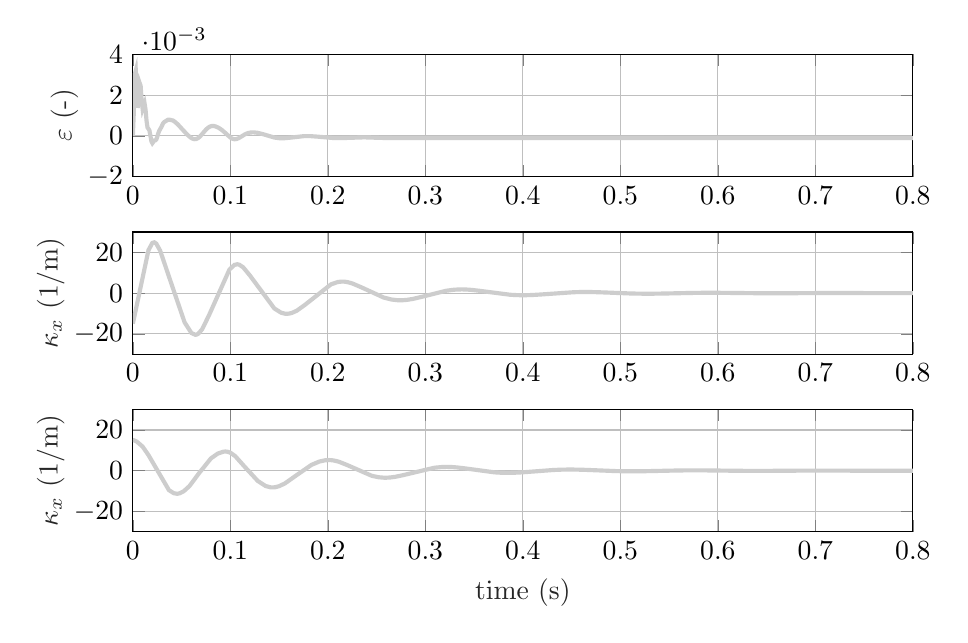
\begin{tikzpicture}

\begin{axis}[%
width=0.817\textwidth,
height=0.128\textwidth,
at={(0\textwidth,0.372\textwidth)},
scale only axis,
xmin=0,
xmax=0.8,
ymin=-0.002,
ymax=0.004,
ylabel style={font=\color{white!15!black}},
ylabel={$\varepsilon$ (-)},
axis background/.style={fill=white},
xmajorgrids,
ymajorgrids,
ylabel style={yshift=-3.5pt}
]
\addplot [color=mycolor1, line width=1.5pt, forget plot]
  table[row sep=crcr]{%
0	0\\
0.00100069999999997	0.00118280000000004\\
0.00200129999999998	0.00302690000000005\\
0.00300199999999995	0.00320659999999995\\
0.00400270000000003	0.00204000000000004\\
0.00500330000000004	0.00137810000000005\\
0.00600400000000001	0.00189989999999995\\
0.00700469999999997	0.00259039999999999\\
0.00800529999999999	0.00244929999999999\\
0.00900599999999996	0.00173400000000001\\
0.010007	0.00132149999999998\\
0.012008	0.0015965\\
0.013009	0.00129559999999995\\
0.014009	0.000752890000000006\\
0.01501	0.000412799999999991\\
0.016011	0.000345240000000024\\
0.017011	0.000263690000000039\\
0.018012	6.14200000004228e-06\\
0.0190129999999999	-0.000267059999999986\\
0.0200129999999999	-0.000355349999999977\\
0.022015	-0.000226130000000047\\
0.023015	-0.000218750000000045\\
0.024016	-0.000179099999999988\\
0.025017	-4.87319999999958e-05\\
0.026017	0.000119230000000026\\
0.027018	0.000247529999999996\\
0.029019	0.000416859999999963\\
0.031021	0.000616460000000041\\
0.032021	0.000675300000000045\\
0.0360240000000001	0.000792470000000045\\
0.038025	0.000790540000000006\\
0.041027	0.000757299999999961\\
0.043029	0.000692970000000015\\
0.046031	0.000568110000000011\\
0.0520350000000001	0.000254760000000021\\
0.056037	5.16750000000288e-05\\
0.059039	-7.46109999999467e-05\\
0.061041	-0.000132119999999958\\
0.063042	-0.00015993999999997\\
0.065043	-0.000150239999999968\\
0.067045	-0.000101770000000001\\
0.0690460000000001	-1.85299999999611e-05\\
0.072048	0.000146179999999996\\
0.0750500000000001	0.000311900000000032\\
0.077051	0.000399240000000023\\
0.079053	0.000458139999999996\\
0.081054	0.000486059999999955\\
0.083055	0.000485100000000016\\
0.085057	0.000460800000000039\\
0.088059	0.000394299999999959\\
0.0910610000000001	0.000299209999999994\\
0.094063	0.000176859999999945\\
0.10007	-8.26600000000122e-05\\
0.10207	-0.000138430000000023\\
0.10407	-0.000163899999999995\\
0.10607	-0.000156939999999994\\
0.10807	-0.000121860000000029\\
0.11107	-3.72770000000022e-05\\
0.11508	7.97289999999728e-05\\
0.11808	0.00013996000000005\\
0.12108	0.000169470000000005\\
0.12408	0.000173120000000027\\
0.12809	0.000150490000000003\\
0.13309	9.08080000000533e-05\\
0.1451	-7.99169999999849e-05\\
0.1501	-0.000113290000000044\\
0.1551	-0.000115599999999993\\
0.16111	-8.87210000000138e-05\\
0.17512	-1.33270000000074e-05\\
0.18212	-1.10450000000428e-05\\
0.19013	-3.9399000000051e-05\\
0.20714	-0.000110049999999973\\
0.21514	-0.000106530000000049\\
0.23716	-7.15239999999895e-05\\
0.25417	-9.7973000000029e-05\\
0.26918	-0.000108980000000036\\
0.36024	-0.000104609999999949\\
0.64943	-0.000108019999999986\\
0.80053	-0.000108019999999986\\
};
\end{axis}

\begin{axis}[%
width=0.817\textwidth,
height=0.128\textwidth,
at={(0\textwidth,0.186\textwidth)},
scale only axis,
xmin=0,
xmax=0.8,
ymin=-30,
ymax=30,
ylabel style={font=\color{white!15!black}},
ylabel={$\kappa_x$ (1/m)},
axis background/.style={fill=white},
xmajorgrids,
ymajorgrids,
ylabel style={yshift=-3.5pt}
]
\addplot [color=mycolor1, line width=1.5pt, forget plot]
  table[row sep=crcr]{%
0	-15\\
0.0160109999999989	21.093\\
0.0200129999999987	24.639\\
0.0220149999999997	24.921\\
0.0240159999999996	24.275\\
0.0280190000000005	20.825\\
0.0370249999999999	8.0954\\
0.0530350000000013	-14.326\\
0.0600400000000008	-19.584\\
0.0640430000000016	-20.462\\
0.0650429999999993	-20.405\\
0.0670450000000002	-19.956\\
0.0710470000000001	-17.783\\
0.0780519999999996	-10.912\\
0.0990660000000005	11.571\\
0.10407	13.835\\
0.10707	14.162\\
0.109069999999999	13.96\\
0.11308	12.693\\
0.120080000000002	8.6293\\
0.145099999999999	-7.5345\\
0.152100000000001	-9.6423\\
0.156099999999999	-10.114\\
0.158110000000001	-10.154\\
0.16011	-10.071\\
0.16311	-9.7278\\
0.168109999999999	-8.6433\\
0.176120000000001	-5.9078\\
0.203140000000001	4.2835\\
0.210139999999999	5.4359\\
0.21414	5.6507\\
0.215140000000002	5.6544\\
0.217140000000001	5.6043\\
0.22015	5.394\\
0.225149999999999	4.733\\
0.234159999999999	2.8837\\
0.257169999999999	-2.165\\
0.265180000000001	-3.1435\\
0.271180000000001	-3.478\\
0.274180000000001	-3.5186\\
0.275179999999999	-3.5142\\
0.277180000000001	-3.4797\\
0.281189999999999	-3.3144\\
0.287189999999999	-2.8582\\
0.296199999999999	-1.8413\\
0.321210000000001	1.1479\\
0.329219999999999	1.6489\\
0.334219999999998	1.7913\\
0.337219999999999	1.8136\\
0.339230000000001	1.8034\\
0.342230000000001	1.7526\\
0.34723	1.5834\\
0.355239999999998	1.144\\
0.387260000000001	-0.82525\\
0.394259999999999	-0.9984\\
0.39827	-1.0371\\
0.400269999999999	-1.0405\\
0.402270000000001	-1.0338\\
0.405270000000002	-1.0058\\
0.410270000000001	-0.91602\\
0.418279999999999	-0.684049999999999\\
0.452300000000001	0.438210000000002\\
0.458310000000001	0.51538\\
0.462309999999999	0.53706\\
0.464310000000001	0.53923\\
0.467310000000001	0.53219\\
0.471309999999999	0.504999999999999\\
0.477319999999999	0.431660000000001\\
0.48732	0.250540000000001\\
0.510339999999999	-0.179390000000001\\
0.518350000000002	-0.263059999999999\\
0.524349999999998	-0.29299\\
0.527349999999998	-0.2974\\
0.530349999999999	-0.295110000000001\\
0.53436	-0.28246\\
0.54036	-0.245730000000002\\
0.54937	-0.161860000000001\\
0.575379999999999	0.0987620000000007\\
0.583390000000001	0.141269999999999\\
0.589390000000002	0.155419999999999\\
0.593399999999999	0.156510000000001\\
0.5974	0.151420000000002\\
0.602399999999999	0.137350000000001\\
0.610410000000002	0.101030000000002\\
0.643429999999999	-0.0701439999999991\\
0.65043	-0.0844270000000016\\
0.655439999999999	-0.0876699999999992\\
0.660440000000001	-0.0854430000000015\\
0.666440000000001	-0.0764409999999991\\
0.67445	-0.0562310000000004\\
0.707470000000001	0.0381\\
0.715479999999999	0.0465310000000017\\
0.72148	0.0475339999999989\\
0.728490000000001	0.0435039999999987\\
0.737490000000001	0.0319460000000014\\
0.773520000000001	-0.0228089999999987\\
0.78152	-0.0262239999999991\\
0.789529999999999	-0.0253240000000012\\
0.799530000000001	-0.0192890000000006\\
0.800529999999998	-0.0184619999999995\\
};
\end{axis}

\begin{axis}[%
width=0.817\textwidth,
height=0.128\textwidth,
at={(0\textwidth,0\textwidth)},
scale only axis,
xmin=0,
xmax=0.8,
xlabel style={font=\color{white!15!black}},
xlabel={time (s)},
ymin=-30,
ymax=30,
ylabel style={font=\color{white!15!black}},
ylabel={$\kappa_x$ (1/m)},
axis background/.style={fill=white},
xmajorgrids,
ymajorgrids,
ylabel style={yshift=-3.5pt}
]
\addplot [color=mycolor1, line width=1.5pt, forget plot]
  table[row sep=crcr]{%
0	15\\
0.00100070000000052	14.95\\
0.00400269999999914	14.297\\
0.0100069999999999	11.814\\
0.0160110000000007	7.6573\\
0.0370249999999999	-9.5688\\
0.0420280000000002	-11.059\\
0.0450300000000006	-11.31\\
0.0460309999999993	-11.287\\
0.0480319999999992	-11.09\\
0.0520350000000001	-10.147\\
0.0580390000000008	-7.5546\\
0.0680449999999997	-1.1197\\
0.0800529999999995	6.0245\\
0.0870580000000007	8.3962\\
0.0930619999999998	9.3567\\
0.0950629999999997	9.4097\\
0.0970650000000006	9.3007\\
0.100070000000001	8.8078\\
0.10507	7.1137\\
0.11408	2.2559\\
0.12809	-5.0254\\
0.136089999999999	-7.5037\\
0.14109	-8.152\\
0.1431	-8.2116\\
0.1441	-8.1999\\
0.146100000000001	-8.0963\\
0.1501	-7.5893\\
0.1561	-6.1972\\
0.167109999999999	-2.4697\\
0.183120000000001	2.8362\\
0.191129999999999	4.4719\\
0.19713	5.1057\\
0.201129999999999	5.2204\\
0.203139999999999	5.1825\\
0.20614	5.008\\
0.21114	4.4251\\
0.219150000000001	2.9017\\
0.24516	-2.5238\\
0.25217	-3.2225\\
0.25717	-3.4262\\
0.259169999999999	-3.4404\\
0.26117	-3.4181\\
0.26418	-3.3202\\
0.26918	-3.0039\\
0.27718	-2.1924\\
0.30921	1.4497\\
0.31621	1.7737\\
0.320209999999999	1.8472\\
0.32221	1.8539\\
0.32422	1.8412\\
0.327220000000001	1.7872\\
0.33222	1.6127\\
0.34023	1.1607\\
0.37125	-0.826919999999999\\
0.37825	-1.0173\\
0.38326	-1.0668\\
0.384259999999999	-1.0684\\
0.387259999999999	-1.0571\\
0.391260000000001	-1.0076\\
0.397259999999999	-0.869759999999999\\
0.406269999999999	-0.56235\\
0.431290000000001	0.34328\\
0.43929	0.500870000000001\\
0.4453	0.555770000000001\\
0.4483	0.56293\\
0.4513	0.557230000000001\\
0.455299999999999	0.53106\\
0.461309999999999	0.457409999999999\\
0.47031	0.29191\\
0.495329999999999	-0.195040000000001\\
0.50334	-0.27852\\
0.50934	-0.30663\\
0.51234	-0.30972\\
0.51534	-0.30593\\
0.519349999999999	-0.290929999999999\\
0.52535	-0.25001\\
0.535360000000001	-0.14809\\
0.55837	0.0959800000000008\\
0.566380000000001	0.144310000000001\\
0.572380000000001	0.16215\\
0.57638	0.165240000000001\\
0.58039	0.1617\\
0.58539	0.14888\\
0.59239	0.11825\\
0.6044	0.0460480000000008\\
0.62041	-0.0462399999999992\\
0.62942	-0.0787340000000007\\
0.63542	-0.0896410000000003\\
0.64043	-0.092041\\
0.645429999999999	-0.0887689999999992\\
0.652430000000001	-0.0760450000000006\\
0.661440000000001	-0.0497449999999997\\
0.68746	0.0322759999999995\\
0.695460000000001	0.0455330000000007\\
0.70247	0.0501120000000004\\
0.70847	0.049004\\
0.715479999999999	0.0426590000000004\\
0.725479999999999	0.0269060000000003\\
0.7525	-0.0191949999999999\\
0.761509999999999	-0.0263190000000009\\
0.76951	-0.0276610000000002\\
0.777520000000001	-0.0247609999999998\\
0.78853	-0.0157760000000007\\
0.80053	-0.00321839999999973\\
};
\end{axis}
\end{tikzpicture}%
  \vspace{-3mm}
  \caption{Three-dimensional volumetric evolution of the one-link soft robot model with initial conditions $\q_0 = (0 , -15, 15)^\top$ and $\dq_0 = (0, 2500, 0)^\top$. Notice that the soft robot oscillates about the set of stable equilibria $\Omega_{\textrm{stab}}$. }
  \label{fig:C2:natural_states}
\end{figure}
%
%
\begin{figure}[!t]
  %\vspace{-3mm}
  \centering
  % This file was created by matlab2tikz.
%
%The latest updates can be retrieved from
%  http://www.mathworks.com/matlabcentral/fileexchange/22022-matlab2tikz-matlab2tikz
%where you can also make suggestions and rate matlab2tikz.
%
\begin{tikzpicture}

\begin{axis}[%
width=0.216\textwidth,
height=0.199\textwidth,
at={(0\textwidth,0.253\textwidth)},
scale only axis,
axis on top,
xmin=0.5,
xmax=522.5,
tick align=outside,
y dir=reverse,
ymin=0.5,
ymax=458.5,
axis line style={draw=none},
ticks=none,
ylabel style={yshift=-7.5pt}
]
\addplot [forget plot] graphics [xmin=0.5, xmax=522.5, ymin=0.5, ymax=458.5] {fig_C2_natural_3D-1.png};
\end{axis}

\begin{axis}[%
width=0.216\textwidth,
height=0.199\textwidth,
at={(0.245\textwidth,0.253\textwidth)},
scale only axis,
axis on top,
xmin=0.5,
xmax=522.5,
tick align=outside,
y dir=reverse,
ymin=0.5,
ymax=458.5,
axis line style={draw=none},
ticks=none,
ylabel style={yshift=-7.5pt}
]
\addplot [forget plot] graphics [xmin=0.5, xmax=522.5, ymin=0.5, ymax=458.5] {fig_C2_natural_3D-2.png};
\end{axis}

\begin{axis}[%
width=0.216\textwidth,
height=0.199\textwidth,
at={(0.49\textwidth,0.253\textwidth)},
scale only axis,
axis on top,
xmin=0.5,
xmax=522.5,
tick align=outside,
y dir=reverse,
ymin=0.5,
ymax=458.5,
axis line style={draw=none},
ticks=none,
ylabel style={yshift=-7.5pt}
]
\addplot [forget plot] graphics [xmin=0.5, xmax=522.5, ymin=0.5, ymax=458.5] {fig_C2_natural_3D-3.png};
\end{axis}

\begin{axis}[%
width=0.216\textwidth,
height=0.199\textwidth,
at={(0.734\textwidth,0.253\textwidth)},
scale only axis,
axis on top,
xmin=0.5,
xmax=522.5,
tick align=outside,
y dir=reverse,
ymin=0.5,
ymax=458.5,
axis line style={draw=none},
ticks=none,
ylabel style={yshift=-7.5pt}
]
\addplot [forget plot] graphics [xmin=0.5, xmax=522.5, ymin=0.5, ymax=458.5] {fig_C2_natural_3D-4.png};
\end{axis}

\begin{axis}[%
width=0.216\textwidth,
height=0.199\textwidth,
at={(0\textwidth,0\textwidth)},
scale only axis,
axis on top,
xmin=0.5,
xmax=522.5,
tick align=outside,
y dir=reverse,
ymin=0.5,
ymax=458.5,
axis line style={draw=none},
ticks=none,
ylabel style={yshift=-7.5pt}
]
\addplot [forget plot] graphics [xmin=0.5, xmax=522.5, ymin=0.5, ymax=458.5] {fig_C2_natural_3D-5.png};
\end{axis}

\begin{axis}[%
width=0.216\textwidth,
height=0.199\textwidth,
at={(0.245\textwidth,0\textwidth)},
scale only axis,
axis on top,
xmin=0.5,
xmax=522.5,
tick align=outside,
y dir=reverse,
ymin=0.5,
ymax=458.5,
axis line style={draw=none},
ticks=none,
ylabel style={yshift=-7.5pt}
]
\addplot [forget plot] graphics [xmin=0.5, xmax=522.5, ymin=0.5, ymax=458.5] {fig_C2_natural_3D-6.png};
\end{axis}

\begin{axis}[%
width=0.216\textwidth,
height=0.199\textwidth,
at={(0.49\textwidth,0\textwidth)},
scale only axis,
axis on top,
xmin=0.5,
xmax=522.5,
tick align=outside,
y dir=reverse,
ymin=0.5,
ymax=458.5,
axis line style={draw=none},
ticks=none,
ylabel style={yshift=-7.5pt}
]
\addplot [forget plot] graphics [xmin=0.5, xmax=522.5, ymin=0.5, ymax=458.5] {fig_C2_natural_3D-7.png};
\end{axis}

\begin{axis}[%
width=0.216\textwidth,
height=0.199\textwidth,
at={(0.734\textwidth,0\textwidth)},
scale only axis,
axis on top,
xmin=0.5,
xmax=522.5,
tick align=outside,
y dir=reverse,
ymin=0.5,
ymax=458.5,
axis line style={draw=none},
ticks=none,
ylabel style={yshift=-7.5pt}
]
\addplot [forget plot] graphics [xmin=0.5, xmax=522.5, ymin=0.5, ymax=458.5] {fig_C2_natural_3D-8.png};
\end{axis}

\begin{axis}[%
width=0.969\textwidth,
height=0.51\textwidth,
at={(-0.01\textwidth,-0.029\textwidth)},
scale only axis,
xmin=0,
xmax=1,
ymin=0,
ymax=1,
axis line style={draw=none},
ticks=none,
axis x line*=bottom,
axis y line*=left,
ylabel style={yshift=-7.5pt}
]
\end{axis}
\end{tikzpicture}%
  \vspace{-3mm}
  \caption{State trajectories of one-link soft robot model with initial conditions $\q_0 = (0 , -15, 15)^\top$ and $\dq_0 = (0, 2500, 0)^\top$. The figure shows the elongation strain $\varepsilon$ and the curvatures $\kappa_x$, $\kappa_y$ in the $xz$-plane and $yz$-plane, respectively.}
  \label{fig:C2:natural_3D}
\end{figure}
%
Besides the existence of stable solutions, the numerical simulations perfectly illustrate the coupled dynamics between the elongation and bending of the soft robot. Due to the difference in mechanical stiffness for elongation and bending, we observe high-frequency and low-frequency oscillation for the elongation strain $\varepsilon(t)$, and we observe low-frequent oscillations for the curvatures $\kappa_x(t)$ and $\kappa_y(t)$. Interestingly, the low-frequency oscillations are passed from the curvature dynamics to elongation dynamics; conversely, the dynamics of the elongation barely affect the curvatures. After sufficient time passes, the trajectories indeed tend to the set of stable equilibria $\Omega$.

\subsection{Experimental platform}
\noindent Before validating the one-link dynamic model, we detail the experimental setup and control platform of the soft robotic system. We would like to briefly emphasize that sensing is a challenging topic soft robotics, due large continuous deformations and the presence of sensors that might affect the system's dynamics. As such, a combination of integrated sensors were used to recover an estimate of the states $\q \in \mathcal{Q}$. First of all, we employed a 9-DOF inertial measurement unit (Bosch, BNO055) measures the angular displacement of the soft robot's end-effector (i.e., $\sigma = L$). Through on-board sensor fusion, the bending angle of the soft robot can be recovered, i.e., $\beta = \kappa l$. Since the bending angle alone is not sufficient to decouple the curvature and elongation, additional sensing is required. Consequently, we used a vision sensor (\texttt{CreateLab}, \texttt{PixyCam2}) with an embedded processor (\texttt{NXP LPC44330}, 200 MHz) for optical tracking. A spherical optical marker is attached to the end-effector of the soft robot. Through trigonometry and the measured bending angle $\beta$, an estimate of the position vector $\gammaB(L,\q)$ can be recovered. Given the analytic expressions for the orientation and position in \eqref{eq:C2:phi_exact} and \eqref{eq:C2:pos_vector}, an inverse Jacobian kinematic solver is employed to recover an estimate of the state vector $\tvec{q}_d$.
During each experimental trail, it was made sure the soft robotic body does not occlude the optical marker.

As for the pneumatic actuation, an array of proportional-pressure regulators (Festo, VEAB-B-D16) was used with an active pressure range of $-0.1 \;\text{MPa}\, < \uB(t) \le 0.1 \; \textrm{MPa}$, which simultaneously allow for pressure measurements. These measurements are fed into the (quasi-static) model to also recover a quasi-static estimate of the states $\hat{q}_s$. Then, the dynamic estimates $\tvec{q}_{\textrm{dyn}}$ and the quasi-static pressure-based estimates $\tvec{q}_{\textrm{qs}}$ are fused using a complementary filter. The control and data acquisition are done using a \texttt{Raspberry Pi 4} (\texttt{2GB}). The full experimental setup can be seen in Figure \ref{fig:5}.

\begin{example}[Model validation -- unforced, forced, and external loads]
\noindent To validate the dynamic model, the solutions of the model are compared with measurements of the physical system in unforced,  forced, and tip-load conditions. As such, the model validation is separated into three parts: \textit{i)} unforced, \textit{ii)} forced conditions, and \textit{i)} external tip-loads applied on the end-effector. We start with the unforced scenario, \ie, no input is considered $u_i(t) \equiv 0$. For the unforced analysis, two experimental trails are performed for the unforced validation. First, the soft robot is deformed slightly and then released from rest, which corresponds to the initial conditions $\q_0 = \left(\;0.015,\,4.75,\,0\; \right)^\top$ and $\dq_0 = 0_3$. Since the mechanical deformations are relatively small here, the presence of hyper-elastic and visco-elastic material behavior are less dominant. Secondly, the soft robot is moderately deformed such that the initial configuration (or shortly after) lies within the hyper-elastic and visco-elastic regime. In this scenario, the nonlinear and time-dependent material effects may not be neglected. These initial conditions correspond to $\q_0 = \left(\;0.046,\,11.25,\,0\; \right)^\top$ and $\dot{{q}}_0 = 0_3$. It is worth mentioning that the creep strains $\lambda$ are difficult to distinguish from the true strain, and thus the initial conditions for $\lambda(t_0)$ are determined empirically. The validation results for both unforced scenario are shown in Figure \ref{fig:6}a. The associated code for the unforced validation simulations can be found under \texttt{./valid\_one\_link\_open.m}.
\end{example}

%
\begin{figure}[!t]
\centering
%\includegraphics[width = 0.95\textwidth]{CaasenbroodFig6.eps}
\caption{\textbf{(a)} Validation results of the
dynamic model in unforced conditions, where the dashed lines represent the experimental measurements and the solid lines are the simulated trajectories. \textbf{(b)} Validation results of the dynamic model in forced conditions, where the dashed lines represent the experimental data from the inertial sensor and the solid lines simulated. In addition, the figure also illustrates the model for Hookean elasticity and applied pressure inputs $u(t)$ to the dynamical system. It is evident from these comparison results that FEM-driven elasticity models can significantly improve accuracy. \textbf{(c)} Experimental validation of the one-link soft robot subjected to various end-effector payloads of different mass $m_\delta = \{0.05,\,0.1,\,0.15\}$ kg. \textbf{(d)} The quasi-static deformation produced by the hyper-elastic model under various end-effector loads. In both figures, the solid lines represent the dynamic model and the dashed lines are the experimental measurements. \label{fig:6}}
\end{figure}
%
As can be seen, the state trajectories of the end-effector closely match the ground truth trajectories, even for significant nonlinear deformation. For the first validation run (inside linear elastic regime), the RMS error and the maximum error are $\pm0.19$ and $\pm 0.50$ degrees, respectively. For the second case (outside the linear elastic regime), the RMS error and the maximum error is $\pm0.78$ and $\pm 2.33$ degrees, respectively.

Second, we consider a forced scenario in which a regulated pressure input is applied to the pneumatic bellows. Since the pneumatic mapping $H$ in \eqref{eq:mapping_H} plays an important role here, the actuator coefficients are recomputed to match the experimental data better. To be more specific, by considering a pre-defined set of excitation signals $u(t)$ of various amplitudes and frequencies, a least-squares optimization routine is employed that minimizes the difference between the measured states $\hat{q}$ with the simulated states ${q}$ by tuning the coefficients $\alpha_\varepsilon$ and $\alpha_\kappa$. This leads to the following values: $\alpha_\varepsilon = 2.34\cdot 10^{-7}$ and $\alpha_\kappa =  1.61\cdot 10^{-8}$. As for the excitation signal, we have chosen the following input:
%
\begin{equation}
u_i(t) = P_0 + P_A \left[\frac{1}{2} + \frac{1}{2}\sin(t + \phi_i) \right]\cdot \max(0.05t,1),
\end{equation}
%
with a static offset $P_0 = 10$ kPa, an amplitude $P_A = 25$ kPa, and a phase offset $\phi_i = (i-1)\frac{2\pi}{m}$ rad. To highlight the significance of the proposed hyper-elastic modeling approach, we also compare the results using an optimized Hookean material material model with $k_e = 50.6$ N/m and $k_b = 5.8\cdot 10^{-4}$ Nm/rad. The initial conditions are set to zero. The validations results for both the FEM-driven hyper-elasticity model and linear model in the forced setting are shown in Figure \ref{fig:6}b. The figure also shows the measured outputs from the pneumatic VEAB regulators $u_i(t)$, which are directly fed into both linear and hyper-elastic models. The associated code for the forced validation can be found under \texttt{./valid\_one\_link\_closed.m}.

Given these results, two key observations can be made. First, both the linear Hookean and hyper-elastic models provide reasonable accuracy for small deformations $0 \le \kappa(t) \le 3$ with a RMS error of $\pm0.13$ and $\pm0.16$ in curvature, respectively. However, as deformations exceed the linear regime, the hyper-elastic model significantly outperforms the Hookean model. Focusing on the hyper-elastic model, both the asymmetric stiffness in radial direction and the strain-hardening are captured well, where the the linear models is not sufficiently rich to capture the material effects. The overall RMS errors for the linear and hyper-elastic model are $\pm1.79$ and $\pm0.21$ in curvature, respectively. Regarding the end-effector accuracy, the overall RMS errors for the linear and hyper-elastic model are $\pm2.58$ and $\pm0.65$ mm, respectively; which translates to an arc-length normalized error of $\pm4.09\%$ and $\pm1.03\%$. These validations results show that introducing nonlinear elastic effects driven by FEM-data can further improve the accuracy for a larger region of the soft robot's workspace.

For the last validation case, we subject the soft robot to an external payload of mass $\delta_m$ located at the end-effector. To model the disturbance, we use the expression for the external payload disturbance model $\delta_m$ in \eqref{eq:delta_payload}. The goal here is \textit{i)} to demonstrate the accuracy of the proposed payload model and quasi-static behavior of the dynamic model, and \textit{ii)} to highlight the limitations of the PCC assumptions under certain conditions. In this analysis, we consider three different payloads $m_\delta = \{0.05,\,0.1,\,0.15\}$ kg.
The experimental results of the payloads deformations are shown in Figure \ref{fig:6}c, and the resulting quasi-static deformations of the dynamic model are shown in Figure \ref{fig:6}d. The associated code for the external payload simulations can be found under \texttt{./valid\_one\_link\_tipload.m}.

As can be seen, the quasi-static behavior of the dynamic model matches the experimental results relatively well for smaller payloads. For the mass $m_\delta = 0.05$ kg, the Euclidean error between the model and the measurement are $\pm1.31$ mm. Increasing the payload to $m_\delta = 0.1$ kg leads to an error of $\pm2.15$ mm. We can also clearly observe that the estimate of the backbone curve subject to the PCC condition is beginning to deviate from the ground truth yet the overall shape still matches the experimental data. Lastly, by further increase the payload $m_\delta = 0.15$ kg, we clearly observe the limitations of the PCC condition under external loads -- with an end-effector error of $3.98$ mm. Also, there is a clear discrepancy in the backbone curve of the model and the ground truth, which might imply the PCC condition is no longer valid here as the payload could induce non-constant curvatures along the backbone. A possible solution might be to introduce a different shape parametrization, similar to the works \cite{Chirikjian1994,Boyer2021,Renda2020,DellaSantina2020}.

\begin{example}[Model benchmark -- Multi-link soft manipulator case]
\noindent In this section, we benchmark the proposed numerical integration scheme for a dynamic model of a six-link soft robot manipulator ($N = 6$). Here, we want to highlight that sufficient numerical speed can be obtained while preserving sufficient numerical precision. This is an important criteria for model-based control, as slow numerical models lack transferability from theory to application. As mentioned earlier, the numerical integration of the Lagrangian entities is the computational bottleneck. Although the MDE solver does aid with numerical performance; ultimately, using a balanced spatial and temporal discretization impacts real-time performance the most. Trivially, using larger stepsize -- both in space and time -- lead to a decrease in numerical precision; and in some cases numerical instability. In this benchmark, we investigate these effects by varying two solver parameters: the spatial stepsize of the explicit MDE solver denoted by $\Delta \sigma$ and the temporal stepsize of the implicit trapezoidal solver denoted by $\Delta t$. For convenience, we represent these stepsizes as standardized parameters: the number of finite elements $N_s = L/\Delta \sigma$ and the implicit solver frequency $f_s = \Delta t\inv$. For the benchmark, we choose a total length of $L = 0.15$ m and simulation time of $T = 10$ s.
\end{example}

%
The extension to the multi-link soft robot ($N = 6$) can be described by a following generalized coordinates with the following structure:
%
\begin{equation}
\q = \left(\,\varepsilon_1,\,\kappa_{x,1},\kappa_{y,1},...,\varepsilon_6,\,\kappa_{x,6},\kappa_{y,6} \, \right)^\top \in \mathcal{Q}
\end{equation}
%
To ensure the soft manipulator is self-supporting, we introduce slight variations to the hyper-elastic stiffness, link lengths, and the inertial properties of the dynamical system. Considering homogeneity, all links are chosen identical in length and mass: intrinsic link length $L_i = 0.025$ m and mass $m_i = 0.05$ kg. Next, the bending stiffness is slightly altered where we choose $\alpha_3 = 0.425$ Nm/rad and $\alpha_4 = 0.4$ Nm/rad. Please note that the material domain is now given by $\Xs = [0,\sum^N_{i=1} L_i]$. To introduce some interesting dynamics for the benchmark, we purely excite the first link of the serial-chain soft robot manipulator with a harmonic input:
%
\begin{align}
u_i(t) = \begin{cases}
P_a \cos(t) & \text{for} \; i = 1, \\
0 & \text{otherwise},
\label{eq:harm_freq}
\end{cases}
\end{align}
%
where $P_a = 125$ kPa is the pressure amplitude. As for the pneumatic mapping that converts pressure to joint torques, we choose $\tau = \left(H \otimes I_6 \right)u $ as the corresponding pneumatic map for the six-link soft manipulator. In total 36 benchmark simulations with different solver settings were performed and tested for their precision relative to a high-precision model ($f_s = 500$ Hz and $N_s = 500$). The state trajectories of the high-precision model are shown in Figure \ref{fig:7}a, whereas Figure \ref{fig:7}b is provided to highlight the underlying dynamics and the trajectory of the end-effector. The results for all benchmark simulations are shown in Table \ref{tab:benchmark_table}. The associated code for the six-link simulations can be found under \texttt{./benchmark\_six\_link.m} on the repository.

%
\begin{figure}[!t]
\centering
%\includegraphics[width =0.475\textwidth]{CaasenbroodFig7.eps}
\caption{\textbf{(a)} State trajectories of six-link soft robot model under dynamic excitation. The figure shows the extensible elongation strains and the total curvature $\kappa = \sqrt{\kappa_x^2 + \kappa_x^2}$ (as the dynamics are planar). \textbf{(b)} The three-dimensional representation of the end-effector trajectory of the six-link soft robot. Notice that the dynamics of the six-link robot converge to a periodic solution. \label{fig:7}}
\end{figure}

Let us first discuss the dynamics of the six-link soft manipulator subjected to a harmonic input. Given this relatively straightforward harmonic excitation, some interesting (stable) nonlinear dynamics appear. Although we excite the system using one harmonic, the dynamics of the soft robot show a rich collection of harmonic oscillations -- highlighting its nonlinear nature. Furthermore, after a short transient time (i.e., $t < 5$), the solutions of the multi-link soft robotic system tend to a so-called \emph{periodic solution}. Here, a solution is called periodic if there exists a period time $T_c >  0$ such that $\q(t) = \q(t + T_c)$ for all time $t$. Similar observations of the existence of periodic solutions (and control of such oscillations) were reported by Della Santina et al. \cite{Santina2021} for articulated soft robots. Given the harmonic excitation in \eqref{eq:harm_freq}, the period time here is $T_c = 1$.

Now, we can exploit these periodic solutions for benchmarking the numerical solver in which we compare the solution of a high-resolution model (i.e., ground truth) to the benchmark solution. Let us define the benchmark error as the Euclidean distance between the two periodic solutions:
%
\begin{align}
e & = \int^{T_c}_0 || \,^0\hat{p}(q(t),L) - \,^0p(q(t),L) || \; dt, \notag \\ & \approx \frac{1}{W}\sum_{i = 1}^{W} || \,^0\hat{p}(q(t_i),L) - \,^0p(q(t_i),L)) ||,
\end{align}
%
where $W$ is the number of time samples of the benchmark model inside the time interval of the periodic solution, and $^0\hat{p}(\cdot,L)$ and $^0p(\cdot,L)$ the tip position of the benchmark and the ground truth, respectively. The index $W$ naturally depends on the sampling frequency of the implicit solver. Table 2 shows the normalized errors (i.e., the tracking error $e$ normalized with the manipulator length $L$) together with the effective computation times of the numerical solver.
\clearpage


\begin{sidewaystable}[!t]
% \begin{landscape}
% \begin{table}
\caption{Benchmark results of the six-link soft robot manipulator for various temporal and spatial discretizations ($T =10$ s). The tables shows the mean tracking error of the end-effector relative to a ground truth ($f_s = 500$ Hz and $N_s = 500$ elements). The RMS errors are normalized with the total length $L = 0.15$ (i.e., the errors are presented in $\%$). The CPU times are also given; where the light-gray entries achieve real-time computation (consistently).  \label{tab:benchmark_table}}
\centering

\begin{tabular}{l|lllllll}
%\toprule
$N = 6$ s  & $N_s = 24$ & $N_s =36$ &  $N_s =60$ &  $N_s = 90$ & $N_s = 120$ & $N_s =180$ \\[0.15em]
%\midrule
$f_s = 25$ Hz &  \textcolor{deepcolor}{\small{19.0 / 1.77s }} &  \textcolor{deepcolor}{\small{9.37 / 2.54s }} & \textcolor{deepcolor}{\small{5.36 / 4.06s }} &  \textcolor{deepcolor}{\small{4.63 / 5.98s }} &  \textcolor{deepcolor}{\small{4.62 / 7.93s}} & \small{4.43 / 11.75s } \\ [0.5em]
$f_s = 50$ Hz &  \textcolor{deepcolor}{\small{17.5 / 3.50s }} &  \textcolor{deepcolor}{\small{7.04 / 5.04s }} &  \textcolor{deepcolor}{\small{4.33 / 6.73s}} & \small{3.69 / 11.60s } & \small{3.60 / 15.3s} & \small{3.69 / 22.71s } \\ [0.5em]
$f_s = 75$ Hz &  \textcolor{deepcolor}{\small{13.77 / 5.31s}} &  \textcolor{deepcolor}{\small{5.80 / 7.56s}} & \small{4.51 / 12.41s} & \small{4.22 / 17.49s} & \small{3.68 / 22.35s} & \small{3.72 / 33.33s} \\ [0.5em]
$f_s = 100$ Hz &  \textcolor{deepcolor}{\small{14.73 / 6.48s}} &  \textcolor{deepcolor}{\small{6.12 / 9.10s}} & \small{4.42 / 14.54s} & \small{3.71 / 21.46s} & \small{3.53 / 28.35s} & \small{2.89 / 42.03s} \\ [0.5em]
$f_s = 150$ Hz &  \textcolor{deepcolor}{\small{15.22 / 7.26s}} &  \textcolor{deepcolor}{\small{5.73 / 9.78s}} & \small{4.32 / 15.58s} & \small{3.46 / 23.07s} & \small{3.16 / 30.38s } & \small{2.67 / 45.06s } \\ [0.5em]
$f_s = 250$ Hz & {\small{14.61 / 11.98s}} & \small{5.32 / 16.71s} & \small{4.14 / 27.11s} & \small{3.35 / 40.19s} & \small{2.86 / 53.06s } & \small{2.21 / 78.61s } \\[0.5em]
%\bottomrule
\end{tabular}
\end{sidewaystable}
%\begin{landscape}

\clearpage
The benchmark table above gives some useful insight into which settings benefit numerical precision and speed the most. First, regarding the coarser models $N = 24$ (i.e., 4 elements per link), we observe large numerical errors of $>\!10\%$ independent of solver frequency. Although one could argue these settings grantee real-time performance (2s of simulation time for 1s computation at $N_s = 24$, $f_s = 75$ Hz) and might suffice for model-based control in slow settings (i.e., set-point stabilization), they are most likely unsuited for dynamic tracking objectives. Moving towards $N_s = 60$ (i.e., 10 elements per link), we observe a significant improvement in numerical precision $\pm4\%$ and while still retaining real-time performance (1.6s of simulation time for 1s computation time at $f_s = 50$ Hz). As such, these settings show that both numerical precision and real-time computation can be achieved for more complicated multi-links soft robots. However, regarding the high-accuracy models $N_s > 100$, we see only a slight increase in numerical precision $\pm3\%$ yet lose real-time capabilities. Consequently, these models might be suited for offline simulations, but lack transferability to online model-based control. However, a possible solution here might be to convert the \texttt{MATLAB} model into a \texttt{C} or \texttt{C++} equivalent model to further increase numerical speed \cite{Grazioso2019,Sadati2020}.

\begin{example}[Closed-loop control -- Passivity-based controller under material certainty and mass disturbance]
\noindent In the last numerical analysis, we demonstrate the results of the proposed passivity-based adaptive scheme. Due to its compactness and computational speed, we again consider the model of the one-link soft robot as seen in previous simulations. To illustrate the robustness of the controller, we purposely introduce some uncertainties. First, we introduce uncertainties in the hyper-elastic material parameters that deviate moderately from their true values in Table 1. Second, we introduce a payload to the end-effector of mass $m_\delta = 0.1$ kg. We again model this external disturbance using the relation in \eqref{eq:delta_payload}. Following the linear parametrizability of the uncertainties, the parameter estimation vector yields:
\end{example}
%
\begin{equation}
\tvec{\pi}(t) = \left( \tilde{\alpha}_1,\,\tilde{\alpha}_2,\,\tilde{\alpha}_4,\, \tilde{\alpha}_5,\, \tilde{m}_\delta\right)^\top,
\end{equation}
%
with initial conditions $\tvec{\pi}(t_0) = \tvec{\pi}_0 = \left(0.75 {\alpha}_1,\,0.75{\alpha}_2,\,0.45{\alpha}_4,\, 0.45{\alpha}_5,\, 0.65{m}_\delta\right)^\top$. Furthermore, the feedback gains and the adaptation rate are chosen as diagonal matrices as follows $K_p = \text{diag}(5,5\text{e-}5,5\text{e-}5)
$, $K_d = \text{diag}(1,1\text{e-}5,1\text{e-}5)$, $\Lambda = I_3$, and $K_\Pi =  \text{diag}(5\text{e}3,5\text{e}3,2\text{e-}6,2\text{e-}6,2\text{e-}2)$. These values were found to yield the best performance while avoiding noticeable oscillations in the closed-loop dynamics. Lastly, the following reference trajectory is considered:
%
\begin{equation}
\q_d(t) = \left(0.01 + 0.01\,\sin(t),\, 30 \,\sin(t),\, 30 \,\cos(t)\right)^\top,
\end{equation}
%
Since the reference trajectory above satisfies persistence of
excitation (see Remark 2), it should grantee the all convergence of the hyper-elastic material estimation and the unknown mass contribution. Figure \ref{fig:8}a shows the state trajectories of the soft robot, Figure \ref{fig:8}b is provided to better illustrate the underlying dynamics of the controller, and Figure \ref{fig:9} shows the evolution of the nonlinear stiffnesses estimates, $\hat{k}_e(q,\hat{\Pi})$ and $\hat{k_b}(q,\hat{\Pi})$, respectively; and the payload estimate $\hat{m}_\delta(\hat{\Pi})$.

%
\begin{figure}[!t]
  \vspace{-5mm}
  \centering
  % This file was created by matlab2tikz.
%
\definecolor{mycolor1}{rgb}{0.80392,0.80392,0.80392}%
\definecolor{mycolor2}{rgb}{0.00000,0.34510,0.65882}%
%
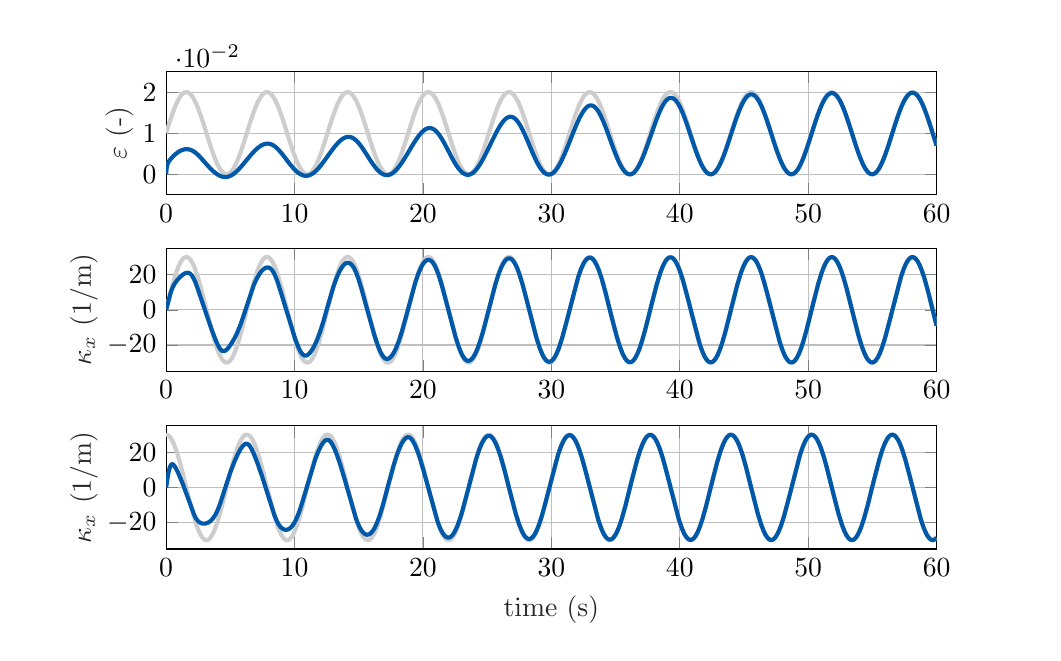
\begin{tikzpicture}

\begin{axis}[%
width=0.807\textwidth,
height=0.129\textwidth,
at={(0\textwidth,0.371\textwidth)},
scale only axis,
xmin=0,
xmax=60,
ymin=-0.005,
ymax=0.025,
ylabel style={font=\color{white!15!black}},
ylabel={$\varepsilon$ (-)},
axis background/.style={fill=white},
xmajorgrids,
ymajorgrids,
ylabel style={yshift=-3.5pt}
]
\addplot [color=mycolor1, line width=1.5pt, forget plot]
  table[row sep=crcr]{%
0	0.00999999999999801\\
0.175069999999998	0.0117419999999981\\
0.275109999999998	0.0127170000000021\\
0.375160000000001	0.0136639999999986\\
0.450189999999999	0.0143509999999978\\
0.525219999999997	0.0150140000000007\\
0.600250000000003	0.0156479999999988\\
0.650269999999999	0.0160539999999969\\
0.725299999999997	0.0166340000000034\\
0.775320000000001	0.0169989999999984\\
0.825339999999997	0.0173479999999984\\
0.875360000000001	0.0176779999999965\\
0.92539	0.017989\\
0.975409999999997	0.0182789999999997\\
1.0254	0.0185490000000001\\
1.0754	0.0187979999999968\\
1.1255	0.0190249999999992\\
1.1755	0.0192290000000028\\
1.2255	0.0194100000000006\\
1.2755	0.0195670000000021\\
1.3256	0.0197009999999977\\
1.3756	0.0198099999999997\\
1.4256	0.0198949999999982\\
1.4756	0.0199550000000031\\
1.5256	0.01999\\
1.5757	0.0200000000000031\\
1.6257	0.0199849999999984\\
1.6757	0.0199449999999999\\
1.7257	0.0198800000000006\\
1.7757	0.0197909999999979\\
1.8258	0.0196770000000015\\
1.8758	0.0195390000000017\\
1.9258	0.0193760000000012\\
1.9758	0.0191909999999993\\
2.0258	0.0189820000000012\\
2.0759	0.0187510000000017\\
2.1259	0.0184989999999985\\
2.1759	0.0182239999999965\\
2.2259	0.0179299999999998\\
2.2759	0.0176149999999993\\
2.326	0.0172820000000016\\
2.376	0.0169300000000021\\
2.451	0.016370000000002\\
2.5261	0.0157740000000004\\
2.6011	0.0151460000000014\\
2.6761	0.0144880000000001\\
2.7511	0.0138060000000024\\
2.8262	0.0131020000000035\\
2.9262	0.0121370000000027\\
3.0513	0.0109020000000015\\
3.3764	0.00767340000000161\\
3.4764	0.00671369999999882\\
3.5765	0.00578680000000276\\
3.6515	0.0051187999999982\\
3.7266	0.00447830000000238\\
3.8016	0.00386890000000051\\
3.8516	0.00348160000000064\\
3.9016	0.00311049999999824\\
3.9516	0.00275680000000023\\
4.0017	0.0024210999999994\\
4.0517	0.00210440000000034\\
4.1017	0.00180739999999702\\
4.1517	0.00153099999999995\\
4.2018	0.00127570000000077\\
4.2518	0.00104220000000055\\
4.3018	0.000831169999997883\\
4.3518	0.000643060000001583\\
4.4018	0.000478360000002453\\
4.4519	0.000337469999998063\\
4.5019	0.000220759999997711\\
4.5519	0.000128510000003246\\
4.6019	6.09579999988341e-05\\
4.6519	1.82659999978796e-05\\
4.702	5.43900000593567e-07\\
4.752	7.83619999822349e-06\\
4.802	4.01249999981701e-05\\
4.852	9.73280000025056e-05\\
4.902	0.000179299999999216\\
4.9521	0.000285849999997367\\
5.0021	0.000416690000001552\\
5.0521	0.00057151000000033\\
5.1021	0.00074991000000324\\
5.1521	0.000951450000002296\\
5.2022	0.00117560000000339\\
5.2522	0.00142189999999687\\
5.3022	0.00168959999999885\\
5.3522	0.00197810000000231\\
5.4023	0.00228669999999909\\
5.4523	0.00261449999999996\\
5.5023	0.00296089999999793\\
5.5523	0.00332480000000146\\
5.6023	0.00370550000000236\\
5.6774	0.00430560000000213\\
5.7524	0.0049379000000016\\
5.8274	0.00559859999999901\\
5.9025	0.00628410000000201\\
5.9775	0.0069903999999994\\
6.0775	0.00795790000000096\\
6.2026	0.00919489999999712\\
6.4777	0.0119329999999991\\
6.5777	0.0129030000000014\\
6.6528	0.013612000000002\\
6.7278	0.0143010000000032\\
6.8028	0.0149660000000011\\
6.8779	0.0156020000000012\\
6.9279	0.0160100000000014\\
6.9779	0.0164019999999994\\
7.0279	0.0167780000000022\\
7.0779	0.0171369999999982\\
7.128	0.017477999999997\\
7.178	0.0178009999999986\\
7.228	0.018104000000001\\
7.278	0.018386999999997\\
7.3281	0.0186490000000035\\
7.3781	0.0188890000000015\\
7.4281	0.0191069999999982\\
7.4781	0.0193020000000033\\
7.5281	0.0194740000000024\\
7.5782	0.0196219999999983\\
7.6282	0.0197459999999978\\
7.6782	0.0198460000000011\\
7.7282	0.0199209999999965\\
7.7782	0.0199709999999982\\
7.8283	0.0199969999999965\\
7.8783	0.0199969999999965\\
7.9283	0.0199720000000028\\
7.9783	0.0199229999999986\\
8.0283	0.0198480000000032\\
8.0784	0.0197489999999974\\
8.1284	0.0196260000000024\\
8.1784	0.0194779999999994\\
8.2284	0.0193069999999977\\
8.2784	0.0191129999999973\\
8.3285	0.0188950000000006\\
8.3785	0.018656\\
8.4285	0.0183940000000007\\
8.4785	0.0181120000000021\\
8.5286	0.0178099999999972\\
8.5786	0.0174880000000002\\
8.6286	0.0171470000000014\\
8.6786	0.0167879999999982\\
8.7536	0.0162189999999995\\
8.8037	0.0158190000000005\\
8.8787	0.0151929999999965\\
8.9537	0.0145380000000017\\
9.0288	0.0138570000000016\\
9.1038	0.0131549999999976\\
9.1788	0.0124350000000035\\
9.3039	0.0112060000000014\\
9.654	0.00772760000000261\\
9.7541	0.00676630000000245\\
9.8291	0.00606609999999819\\
9.9041	0.0053880000000035\\
9.9792	0.00473579999999885\\
10.029	0.00431729999999675\\
10.104	0.00371650000000301\\
10.154	0.00333539999999743\\
10.204	0.00297090000000111\\
10.254	0.00262409999999846\\
10.304	0.00229569999999768\\
10.354	0.00198660000000217\\
10.404	0.0016974999999988\\
10.454	0.00142919999999691\\
10.504	0.00118230000000352\\
10.554	0.00095749999999839\\
10.604	0.000755310000002396\\
10.654	0.000576240000000894\\
10.704	0.000420750000003522\\
10.754	0.000289219999999091\\
10.805	0.00018199000000152\\
10.855	9.93129999997677e-05\\
10.905	4.14040000009663e-05\\
10.955	8.40789999756453e-06\\
11.005	4.0598000339287e-07\\
11.055	1.74190000024055e-05\\
11.105	5.94030000016232e-05\\
11.155	0.000126260000001821\\
11.205	0.000217810000002316\\
11.255	0.000333830000002422\\
11.305	0.000474029999999459\\
11.355	0.000638059999999996\\
11.405	0.000825519999999358\\
11.455	0.00103589999999798\\
11.505	0.00126869999999712\\
11.555	0.00152340000000351\\
11.605	0.00179930000000184\\
11.655	0.00209569999999815\\
11.705	0.0024117999999973\\
11.755	0.00274699999999939\\
11.805	0.00310029999999983\\
11.855	0.00347080000000233\\
11.905	0.00385769999999752\\
11.98	0.00446649999999948\\
12.055	0.00510649999999657\\
12.13	0.00577400000000239\\
12.205	0.00646520000000095\\
12.28	0.00717639999999875\\
12.38	0.0081485999999984\\
12.505	0.00938880000000353\\
12.755	0.0118780000000029\\
12.855	0.0128500000000003\\
12.93	0.0135599999999982\\
13.005	0.0142510000000016\\
13.08	0.014916999999997\\
13.13	0.0153469999999984\\
13.18	0.0157620000000023\\
13.306	0.0167369999999991\\
13.381	0.0172719999999984\\
13.431	0.0176060000000007\\
13.481	0.0179210000000012\\
13.531	0.0182160000000025\\
13.581	0.0184909999999974\\
13.631	0.0187450000000027\\
13.681	0.0189760000000021\\
13.731	0.0191850000000002\\
13.781	0.0193719999999971\\
13.831	0.0195340000000002\\
13.881	0.0196729999999974\\
13.931	0.0197879999999984\\
13.981	0.0198779999999985\\
14.031	0.0199440000000024\\
14.081	0.0199840000000009\\
14.131	0.0200000000000031\\
14.181	0.01999\\
14.231	0.0199560000000005\\
14.281	0.0198970000000003\\
14.331	0.0198129999999992\\
14.381	0.0197039999999973\\
14.431	0.0195709999999991\\
14.481	0.0194150000000022\\
14.531	0.0192339999999973\\
14.581	0.0190309999999982\\
14.631	0.0188050000000004\\
14.681	0.0185570000000013\\
14.731	0.0182870000000008\\
14.781	0.0179970000000012\\
14.831	0.0176870000000022\\
14.881	0.017356999999997\\
14.931	0.0170099999999991\\
14.981	0.0166439999999994\\
15.031	0.0162619999999976\\
15.106	0.0156599999999969\\
15.181	0.0150259999999989\\
15.256	0.0143640000000005\\
15.331	0.0136770000000013\\
15.406	0.0129700000000028\\
15.506	0.0120009999999979\\
15.657	0.0105140000000006\\
15.882	0.0082722000000004\\
15.982	0.00729710000000239\\
16.057	0.00658299999999912\\
16.132	0.00588809999999995\\
16.207	0.0052164000000019\\
16.282	0.00457159999999845\\
16.357	0.00395730000000327\\
16.407	0.00356639999999686\\
16.457	0.00319170000000213\\
16.507	0.002834\\
16.557	0.002494200000001\\
16.607	0.00217320000000143\\
16.657	0.00187180000000353\\
16.707	0.00159070000000128\\
16.757	0.00133069999999691\\
16.807	0.00109230000000338\\
16.857	0.000876200000000438\\
16.907	0.000682939999997245\\
16.957	0.00051298999999716\\
17.007	0.000366769999999406\\
17.057	0.000244649999999069\\
17.107	0.000146929999999657\\
17.157	7.38549999965699e-05\\
17.207	2.56149999984245e-05\\
17.257	2.32600000060756e-06\\
17.307	4.04720000091174e-06\\
17.357	3.07740000025092e-05\\
17.407	8.24390000033759e-05\\
17.457	0.000158910000003232\\
17.507	0.00026000999999809\\
17.557	0.00038545999999684\\
17.607	0.000534969999996804\\
17.657	0.000708160000002067\\
17.707	0.00090458999999754\\
17.757	0.00112380000000201\\
17.807	0.00136520000000218\\
17.857	0.00162819999999897\\
17.907	0.00191209999999842\\
17.957	0.00221619999999945\\
18.033	0.00270880000000062\\
18.083	0.00306009999999901\\
18.133	0.00342870000000062\\
18.183	0.0038138000000032\\
18.258	0.00442019999999843\\
18.333	0.00505799999999823\\
18.408	0.00572350000000199\\
18.483	0.00641319999999723\\
18.558	0.00712299999999999\\
18.658	0.00809389999999865\\
18.783	0.00933320000000037\\
19.058	0.0120689999999968\\
19.158	0.0130359999999996\\
19.233	0.0137410000000031\\
19.308	0.0144260000000003\\
19.383	0.0150859999999966\\
19.458	0.0157170000000022\\
19.533	0.0163160000000033\\
19.583	0.0166960000000032\\
19.633	0.0170590000000033\\
19.708	0.0175699999999992\\
19.758	0.0178870000000018\\
19.808	0.018183999999998\\
19.858	0.0184610000000021\\
19.908	0.0187170000000023\\
19.958	0.0189510000000013\\
20.008	0.0191629999999989\\
20.058	0.0193519999999978\\
20.108	0.0195170000000005\\
20.158	0.0196589999999972\\
20.208	0.0197760000000002\\
20.258	0.0198689999999999\\
20.308	0.0199369999999988\\
20.358	0.0199810000000014\\
20.409	0.0199989999999985\\
20.459	0.0199929999999995\\
20.509	0.0199610000000021\\
20.559	0.0199050000000014\\
20.609	0.0198230000000024\\
20.659	0.0197179999999975\\
20.709	0.0195870000000014\\
20.759	0.0194329999999994\\
20.809	0.0192550000000011\\
20.859	0.0190550000000016\\
20.909	0.0188309999999987\\
20.959	0.0185850000000016\\
21.009	0.0183180000000007\\
21.059	0.0180300000000031\\
21.109	0.0177219999999991\\
21.159	0.0173950000000005\\
21.209	0.0170490000000001\\
21.259	0.016686\\
21.309	0.0163060000000002\\
21.384	0.0157060000000016\\
21.459	0.0150739999999985\\
21.534	0.0144140000000021\\
21.609	0.0137289999999979\\
21.684	0.0130229999999969\\
21.784	0.0120560000000012\\
21.884	0.0110680000000016\\
22.234	0.00759269999999646\\
22.334	0.0066354000000004\\
22.409	0.00593889999999675\\
22.484	0.00526539999999898\\
22.559	0.00461839999999825\\
22.634	0.00400170000000344\\
22.684	0.00360919999999965\\
22.734	0.00323259999999692\\
22.784	0.00287300000000101\\
22.885	0.0022080000000031\\
22.935	0.00190440000000081\\
22.985	0.00162100000000009\\
23.035	0.00135850000000204\\
23.085	0.00111770000000178\\
23.135	0.000899140000001353\\
23.185	0.000703319999999508\\
23.235	0.000530750000002911\\
23.285	0.000381859999997403\\
23.335	0.000257040000001041\\
23.385	0.000156590000003121\\
23.435	8.07649999998716e-05\\
23.485	2.97529999997437e-05\\
23.535	3.68229999736513e-06\\
23.585	2.61779999988221e-06\\
23.635	2.65620000021727e-05\\
23.685	7.54559999975868e-05\\
23.735	0.000149180000001081\\
23.785	0.000247539999996604\\
23.835	0.000370300000000157\\
23.885	0.000517150000000299\\
23.935	0.000687720000001946\\
23.985	0.000881589999998766\\
24.035	0.00109830000000244\\
24.085	0.00133720000000181\\
24.135	0.00159779999999898\\
24.185	0.00187950000000114\\
24.235	0.00218139999999778\\
24.285	0.00250290000000319\\
24.335	0.00284320000000093\\
24.385	0.00320130000000063\\
24.435	0.0035765000000012\\
24.485	0.00396769999999691\\
24.56	0.0045825999999991\\
24.635	0.00522790000000128\\
24.71	0.00590009999999808\\
24.785	0.00659530000000075\\
24.86	0.00730970000000042\\
24.96	0.00828510000000193\\
25.11	0.00977720000000204\\
25.236	0.0110260000000011\\
25.361	0.0122590000000002\\
25.461	0.0132199999999969\\
25.536	0.0139210000000034\\
25.611	0.0145989999999969\\
25.686	0.0152519999999967\\
25.761	0.0158750000000012\\
25.811	0.0162720000000007\\
25.861	0.0166540000000026\\
25.911	0.0170189999999977\\
25.961	0.0173660000000027\\
26.011	0.0176950000000033\\
26.061	0.0180050000000023\\
26.111	0.0182950000000019\\
26.161	0.0185630000000003\\
26.211	0.0188109999999995\\
26.261	0.0190359999999998\\
26.311	0.0192389999999989\\
26.361	0.0194189999999992\\
26.411	0.0195750000000032\\
26.461	0.0197069999999968\\
26.511	0.0198150000000012\\
26.561	0.0198990000000023\\
26.611	0.019956999999998\\
26.661	0.0199909999999974\\
26.711	0.0200000000000031\\
26.761	0.0199830000000034\\
26.811	0.0199420000000003\\
26.861	0.0198759999999965\\
26.911	0.0197849999999988\\
26.961	0.0196699999999979\\
27.011	0.0195300000000032\\
27.061	0.0193670000000026\\
27.111	0.0191799999999986\\
27.161	0.018970000000003\\
27.211	0.018737999999999\\
27.261	0.0184840000000008\\
27.311	0.0182089999999988\\
27.361	0.0179130000000001\\
27.411	0.0175970000000021\\
27.461	0.0172629999999998\\
27.511	0.0169100000000029\\
27.561	0.0165399999999991\\
27.637	0.0159540000000007\\
27.687	0.015545000000003\\
27.762	0.0149060000000034\\
27.837	0.0142390000000034\\
27.912	0.0135480000000001\\
28.012	0.0125969999999995\\
28.137	0.0113720000000015\\
28.312	0.00962549999999851\\
28.462	0.00813569999999686\\
28.562	0.00716380000000072\\
28.637	0.00645300000000049\\
28.712	0.00576209999999833\\
28.787	0.00509499999999719\\
28.862	0.0044556\\
28.937	0.00384729999999678\\
28.987	0.00346090000000032\\
29.037	0.0030908000000025\\
29.087	0.00273789999999963\\
29.137	0.00240329999999744\\
29.187	0.00208760000000296\\
29.237	0.00179179999999945\\
29.287	0.00151650000000103\\
29.337	0.00126240000000166\\
29.387	0.00103010000000126\\
29.437	0.000820300000000884\\
29.487	0.000633460000003083\\
29.537	0.000470049999997002\\
29.587	0.000330470000001526\\
29.637	0.000215089999997531\\
29.687	0.000124180000000251\\
29.737	5.79829999978188e-05\\
29.787	1.66530000029752e-05\\
29.837	2.96289996981614e-07\\
29.887	8.95480000195903e-06\\
29.937	4.26069999974743e-05\\
29.987	0.00010117000000065\\
30.038	0.000184490000002313\\
30.088	0.000292369999996822\\
30.138	0.000424529999996537\\
30.188	0.000580650000003402\\
30.238	0.000760319999997705\\
30.288	0.000963120000001538\\
30.338	0.00118849999999782\\
30.388	0.00143599999999822\\
30.438	0.00170479999999884\\
30.488	0.00199440000000095\\
30.538	0.00230410000000347\\
30.588	0.00263300000000299\\
30.638	0.00298029999999727\\
30.688	0.00334519999999827\\
30.738	0.00372670000000141\\
30.788	0.00412390000000329\\
30.863	0.00474700000000183\\
30.938	0.00539959999999695\\
31.013	0.00607819999999748\\
31.088	0.00677879999999931\\
31.188	0.00774040000000298\\
31.313	0.00897299999999746\\
31.638	0.012203999999997\\
31.713	0.0129289999999997\\
31.813	0.0138699999999972\\
31.888	0.0145499999999998\\
31.963	0.0152050000000017\\
32.038	0.0158300000000011\\
32.113	0.0164230000000032\\
32.188	0.0169789999999992\\
32.238	0.0173289999999966\\
32.288	0.0176599999999993\\
32.338	0.0179710000000028\\
32.388	0.0182629999999975\\
32.464	0.0186619999999991\\
32.514	0.0189009999999996\\
32.564	0.0191179999999989\\
32.614	0.0193119999999993\\
32.664	0.019483000000001\\
32.714	0.0196290000000019\\
32.764	0.0197519999999969\\
32.814	0.0198510000000027\\
32.864	0.0199240000000032\\
32.914	0.0199730000000002\\
32.964	0.0199969999999965\\
33.014	0.019995999999999\\
33.064	0.0199700000000007\\
33.114	0.0199190000000016\\
33.164	0.0198439999999991\\
33.214	0.0197429999999983\\
33.264	0.0196180000000012\\
33.314	0.0194699999999983\\
33.364	0.0192970000000017\\
33.414	0.0191009999999991\\
33.464	0.0188830000000024\\
33.514	0.0186419999999998\\
33.564	0.0183800000000005\\
33.614	0.0180959999999999\\
33.664	0.0177929999999975\\
33.714	0.017470000000003\\
33.764	0.0171279999999996\\
33.814	0.016767999999999\\
33.864	0.0163920000000033\\
33.939	0.0157969999999992\\
33.989	0.0153820000000024\\
34.064	0.0147359999999992\\
34.139	0.0140620000000027\\
34.214	0.0133659999999978\\
34.314	0.0124080000000006\\
34.414	0.0114269999999976\\
34.589	0.00968110000000166\\
34.739	0.00819049999999777\\
34.789	0.00770099999999729\\
34.84	0.00721730000000065\\
34.915	0.00650509999999827\\
34.99	0.00581259999999872\\
35.065	0.0051435999999967\\
35.14	0.00450200000000223\\
35.215	0.00389129999999938\\
35.265	0.0035031000000032\\
35.315	0.00313109999999739\\
35.365	0.0027764000000019\\
35.415	0.00243960000000243\\
35.465	0.00212179999999762\\
35.515	0.00182370000000276\\
35.565	0.00154609999999877\\
35.615	0.00128959999999978\\
35.665	0.00105489999999975\\
35.715	0.000842540000000724\\
35.765	0.000653110000001789\\
35.815	0.000487069999998369\\
35.865	0.000344820000002244\\
35.915	0.000226730000001396\\
35.965	0.000133089999998504\\
36.015	6.41259999980548e-05\\
36.065	2.00200000008977e-05\\
36.115	8.80130002656188e-07\\
36.165	6.75329999921814e-06\\
36.215	3.76249999973766e-05\\
36.265	9.3417999998735e-05\\
36.315	0.000173990000000401\\
36.365	0.00027914999999723\\
36.415	0.000408620000001747\\
36.465	0.000562090000002513\\
36.515	0.000739160000001959\\
36.565	0.000939410000000862\\
36.615	0.00116229999999717\\
36.665	0.00140729999999678\\
36.715	0.00167379999999895\\
36.765	0.00196119999999667\\
36.815	0.00226860000000073\\
36.865	0.00259539999999703\\
36.915	0.00294070000000346\\
36.965	0.00330369999999647\\
37.015	0.00368339999999989\\
37.09	0.00428229999999985\\
37.165	0.00491339999999951\\
37.266	0.00579869999999971\\
37.341	0.00649080000000168\\
37.416	0.00720259999999939\\
37.516	0.00817550000000011\\
37.641	0.00941610000000281\\
37.891	0.0119049999999987\\
37.991	0.0128759999999986\\
38.066	0.0135859999999965\\
38.141	0.0142749999999978\\
38.216	0.0149410000000003\\
38.291	0.0155790000000025\\
38.341	0.0159870000000026\\
38.416	0.0165700000000015\\
38.466	0.0169390000000007\\
38.516	0.0172910000000002\\
38.566	0.0176239999999979\\
38.616	0.0179380000000009\\
38.666	0.0182319999999976\\
38.716	0.0185049999999976\\
38.766	0.0187579999999983\\
38.816	0.0189880000000002\\
38.866	0.0191960000000009\\
38.916	0.0193810000000028\\
38.966	0.0195420000000013\\
39.016	0.019680000000001\\
39.066	0.0197929999999999\\
39.116	0.0198820000000026\\
39.166	0.0199459999999974\\
39.216	0.0199860000000029\\
39.266	0.0200000000000031\\
39.316	0.0199890000000025\\
39.366	0.019953000000001\\
39.416	0.0198930000000033\\
39.466	0.0198070000000001\\
39.516	0.0196979999999982\\
39.566	0.019562999999998\\
39.617	0.019404999999999\\
39.667	0.0192240000000012\\
39.717	0.0190190000000001\\
39.767	0.0187919999999977\\
39.817	0.0185430000000011\\
39.867	0.0182720000000032\\
39.917	0.0179809999999989\\
39.967	0.0176689999999979\\
40.017	0.0173389999999998\\
40.067	0.0169899999999998\\
40.117	0.0166240000000002\\
40.192	0.0160440000000008\\
40.267	0.0154289999999975\\
40.342	0.0147850000000034\\
40.417	0.0141130000000018\\
40.492	0.0134180000000015\\
40.567	0.0127039999999994\\
40.667	0.0117290000000025\\
40.817	0.0102369999999965\\
41.017	0.00824529999999868\\
41.117	0.00727080000000058\\
41.192	0.00655729999999721\\
41.267	0.00586320000000029\\
41.342	0.00519239999999854\\
41.417	0.00454859999999968\\
41.492	0.00393549999999721\\
41.542	0.00354560000000248\\
41.592	0.00317170000000289\\
41.642	0.00281499999999824\\
41.692	0.00247619999999671\\
41.742	0.00215620000000172\\
41.792	0.00185590000000246\\
41.842	0.00157600000000002\\
41.892	0.0013171000000014\\
41.942	0.00107990000000058\\
41.992	0.000865050000001588\\
42.068	0.000585780000001535\\
42.118	0.000428939999999045\\
42.168	0.000296040000002051\\
42.218	0.000187420000003158\\
42.268	0.000103340000002561\\
42.318	4.40239999974779e-05\\
42.368	9.61149999767485e-06\\
42.418	1.90539999778139e-07\\
42.468	1.57850000022108e-05\\
42.518	5.63549999981205e-05\\
42.568	0.000121800000002281\\
42.618	0.000211960000001454\\
42.668	0.000326600000001065\\
42.718	0.000465439999999262\\
42.768	0.000628130000002614\\
42.818	0.000814259999998512\\
42.868	0.00102340000000112\\
42.918	0.00125489999999928\\
42.968	0.00150839999999874\\
43.018	0.00178309999999726\\
43.068	0.00207830000000087\\
43.118	0.00239340000000254\\
43.168	0.00272749999999888\\
43.218	0.00307980000000185\\
43.268	0.00344929999999977\\
43.318	0.00383529999999865\\
43.393	0.0044429000000008\\
43.468	0.00508169999999808\\
43.543	0.00574830000000048\\
43.618	0.0064386999999968\\
43.693	0.00714920000000063\\
43.793	0.0081206999999992\\
43.918	0.00936049999999966\\
44.193	0.0120959999999997\\
44.293	0.0130619999999979\\
44.368	0.0137670000000014\\
44.419	0.0142250000000033\\
44.494	0.0148930000000007\\
44.569	0.0155329999999978\\
44.644	0.0161409999999975\\
44.694	0.016528000000001\\
44.744	0.0168990000000022\\
44.794	0.0172519999999992\\
44.844	0.0175869999999989\\
44.894	0.0179040000000015\\
44.944	0.0182000000000002\\
44.994	0.0184759999999997\\
45.044	0.0187310000000025\\
45.094	0.0189639999999969\\
45.144	0.0191739999999996\\
45.194	0.019362000000001\\
45.244	0.019525999999999\\
45.294	0.0196660000000008\\
45.344	0.0197819999999993\\
45.394	0.0198740000000015\\
45.444	0.0199399999999983\\
45.494	0.0199830000000034\\
45.544	0.0200000000000031\\
45.594	0.019992000000002\\
45.644	0.0199590000000001\\
45.694	0.0199009999999973\\
45.744	0.0198180000000008\\
45.794	0.0197110000000009\\
45.844	0.0195799999999977\\
45.894	0.0194240000000008\\
45.944	0.019244999999998\\
45.994	0.0190430000000035\\
46.044	0.0188180000000031\\
46.094	0.0185710000000014\\
46.144	0.0183030000000031\\
46.194	0.0180140000000009\\
46.244	0.0177049999999994\\
46.294	0.0173770000000033\\
46.369	0.016849999999998\\
46.444	0.0162839999999989\\
46.494	0.0158879999999968\\
46.569	0.0152649999999994\\
46.644	0.0146129999999971\\
46.719	0.0139349999999965\\
46.82	0.0129969999999986\\
46.895	0.0122730000000004\\
46.995	0.0112889999999979\\
47.17	0.00954250000000201\\
47.32	0.00805419999999657\\
47.42	0.00708430000000249\\
47.495	0.0063754999999972\\
47.57	0.00568700000000177\\
47.645	0.00502290000000016\\
47.72	0.00438669999999775\\
47.795	0.00378210000000223\\
47.845	0.00339830000000063\\
47.895	0.00303100000000001\\
47.945	0.00268109999999666\\
47.995	0.00234960000000228\\
48.045	0.00203710000000257\\
48.095	0.00174460000000209\\
48.145	0.00147280000000194\\
48.195	0.00122230000000201\\
48.245	0.000993719999996756\\
48.295	0.000787690000002783\\
48.345	0.000604699999996683\\
48.395	0.000445220000003133\\
48.445	0.000309639999997557\\
48.495	0.000198300000000984\\
48.545	0.000111480000001052\\
48.595	4.93989999981181e-05\\
48.645	1.22080000011238e-05\\
48.695	1.82149761940309e-09\\
48.745	1.28109999977255e-05\\
48.795	5.0604999998427e-05\\
48.845	0.000113290000001598\\
48.895	0.000200700000000609\\
48.945	0.000312630000003367\\
48.995	0.000448790000000088\\
49.045	0.000608849999998995\\
49.095	0.000792390000000864\\
49.145	0.000998969999997712\\
49.195	0.00122809999999873\\
49.246	0.0014790999999974\\
49.296	0.00175149999999746\\
49.346	0.00204449999999667\\
49.396	0.0023572999999999\\
49.446	0.00268940000000129\\
49.496	0.0030397000000022\\
49.546	0.00340740000000039\\
49.596	0.00379159999999956\\
49.671	0.00439670000000092\\
49.746	0.00503330000000091\\
49.821	0.00569790000000125\\
49.896	0.00638670000000019\\
49.971	0.00709580000000187\\
50.071	0.00806610000000063\\
50.196	0.00930489999999651\\
50.471	0.0120410000000035\\
50.571	0.0130089999999967\\
50.671	0.0139459999999971\\
50.746	0.0146239999999977\\
50.821	0.0152750000000026\\
50.896	0.0158970000000025\\
50.971	0.0164860000000004\\
51.021	0.0168589999999966\\
51.096	0.0173849999999973\\
51.146	0.0177130000000005\\
51.196	0.0180209999999974\\
51.246	0.0183099999999996\\
51.296	0.018577999999998\\
51.346	0.0188240000000022\\
51.396	0.019047999999998\\
51.446	0.0192499999999995\\
51.496	0.0194279999999978\\
51.546	0.0195829999999972\\
51.596	0.0197140000000005\\
51.647	0.0198200000000028\\
51.697	0.0199029999999993\\
51.747	0.0199599999999975\\
51.797	0.019992000000002\\
51.847	0.0199989999999985\\
51.897	0.0199819999999988\\
51.947	0.0199390000000008\\
51.997	0.0198719999999994\\
52.047	0.0197789999999998\\
52.097	0.0196630000000013\\
52.147	0.019522000000002\\
52.197	0.0193569999999994\\
52.247	0.019168999999998\\
52.297	0.0189579999999978\\
52.347	0.0187250000000034\\
52.397	0.0184700000000007\\
52.447	0.0181929999999966\\
52.497	0.0178960000000004\\
52.547	0.0175800000000024\\
52.597	0.017243999999998\\
52.647	0.0168899999999965\\
52.697	0.0165190000000024\\
52.747	0.0161319999999989\\
52.822	0.0155230000000017\\
52.897	0.0148820000000001\\
52.972	0.0142140000000026\\
53.047	0.0135220000000018\\
53.122	0.0128109999999992\\
53.222	0.0118379999999974\\
53.347	0.0105980000000017\\
53.597	0.00810890000000342\\
53.697	0.00713760000000008\\
53.772	0.00642739999999975\\
53.847	0.00573729999999983\\
53.922	0.00507120000000327\\
53.997	0.00443289999999763\\
54.123	0.0034402\\
54.173	0.00307099999999849\\
54.223	0.00271920000000136\\
54.273	0.00238559999999666\\
54.323	0.00207100000000082\\
54.373	0.00177620000000189\\
54.423	0.00150200000000211\\
54.473	0.00124910000000256\\
54.523	0.00101810000000313\\
54.573	0.000809500000002572\\
54.623	0.000623920000002443\\
54.673	0.000461799999996515\\
54.723	0.000323539999996569\\
54.773	0.000209490000003143\\
54.823	0.000119929999996771\\
54.873	5.50820000029262e-05\\
54.923	1.51139999999828e-05\\
54.973	1.23310002209109e-07\\
55.023	1.01480000012089e-05\\
55.073	4.51630000029013e-05\\
55.123	0.000105079999997315\\
55.173	0.000189749999996991\\
55.223	0.000298960000002069\\
55.273	0.000432439999997314\\
55.323	0.000589849999997227\\
55.373	0.000770809999998789\\
55.423	0.000974849999998639\\
55.473	0.00120150000000052\\
55.523	0.00145009999999957\\
55.573	0.0017201\\
55.623	0.00201080000000076\\
55.673	0.00232150000000075\\
55.723	0.00265149999999892\\
55.773	0.00299979999999778\\
55.823	0.00336560000000219\\
55.873	0.00374800000000164\\
55.923	0.00414609999999982\\
55.998	0.00477029999999701\\
56.073	0.00542389999999671\\
56.148	0.00610329999999948\\
56.223	0.00680460000000238\\
56.323	0.00776700000000119\\
56.499	0.00949889999999698\\
56.724	0.0117410000000007\\
56.849	0.0129549999999981\\
56.924	0.0136630000000011\\
56.999	0.0143500000000003\\
57.074	0.0150130000000033\\
57.149	0.0156479999999988\\
57.224	0.0162499999999994\\
57.274	0.0166329999999988\\
57.324	0.0169989999999984\\
57.374	0.0173470000000009\\
57.424	0.0176769999999991\\
57.474	0.0179880000000026\\
57.524	0.0182789999999997\\
57.574	0.0185490000000001\\
57.624	0.0187979999999968\\
57.674	0.0190240000000017\\
57.724	0.0192279999999982\\
57.774	0.0194090000000031\\
57.824	0.0195670000000021\\
57.874	0.0197009999999977\\
57.924	0.0198099999999997\\
57.974	0.0198949999999982\\
58.024	0.0199550000000031\\
58.074	0.01999\\
58.124	0.0200000000000031\\
58.174	0.0199849999999984\\
58.224	0.0199449999999999\\
58.274	0.0198800000000006\\
58.324	0.0197909999999979\\
58.374	0.0196770000000015\\
58.424	0.0195390000000017\\
58.474	0.0193769999999986\\
58.524	0.0191909999999993\\
58.574	0.0189829999999986\\
58.624	0.0187519999999992\\
58.674	0.0184989999999985\\
58.724	0.018225000000001\\
58.774	0.0179299999999998\\
58.85	0.0174510000000012\\
58.9	0.0171089999999978\\
58.975	0.0165610000000029\\
59.025	0.0161760000000015\\
59.1	0.0155689999999993\\
59.175	0.0149309999999971\\
59.25	0.0142650000000017\\
59.325	0.013575000000003\\
59.425	0.0126240000000024\\
59.525	0.0116470000000035\\
59.675	0.010154\\
59.875	0.00816360000000316\\
59.975	0.00719099999999884\\
60	0.00695189999999712\\
};
\addplot [color=mycolor2, line width=1.5pt, forget plot]
  table[row sep=crcr]{%
0	0\\
0.0250100000000018	0.000948909999998193\\
0.050021000000001	0.00163409999999686\\
0.0750310000000027	0.00204109999999957\\
0.10004	0.00238650000000007\\
0.125050000000002	0.00258379999999647\\
0.150060000000003	0.00279369999999801\\
0.175069999999998	0.00291380000000174\\
0.20008	0.00306900000000354\\
0.225090000000002	0.00316200000000322\\
0.250100000000003	0.00329359999999923\\
0.275109999999998	0.00337760000000031\\
0.300130000000003	0.00349709999999703\\
0.325139999999998	0.00357809999999859\\
0.350149999999999	0.00368960000000129\\
0.375160000000001	0.00376909999999953\\
0.400170000000003	0.00387400000000326\\
0.425179999999997	0.00395180000000295\\
0.450189999999999	0.00405070000000052\\
0.475200000000001	0.00412639999999698\\
0.500210000000003	0.00421949999999782\\
0.525219999999997	0.00429270000000059\\
0.550229999999999	0.00438050000000345\\
0.575240000000001	0.00445090000000192\\
0.600250000000003	0.00453370000000319\\
0.675280000000001	0.00474390000000113\\
0.700290000000003	0.00481769999999671\\
0.900379999999998	0.00530359999999774\\
1.0504	0.00559839999999667\\
1.1755	0.00579450000000037\\
1.2505	0.0058928999999992\\
1.3506	0.0059944999999999\\
1.4506	0.00606359999999739\\
1.5506	0.00609879999999663\\
1.6507	0.00609899999999897\\
1.7257	0.00607500000000272\\
1.8008	0.00603160000000003\\
1.8758	0.00596639999999837\\
1.9508	0.00588110000000341\\
2.0258	0.00577400000000239\\
2.1009	0.00564669999999978\\
2.1759	0.00549850000000163\\
2.2509	0.0053313000000017\\
2.351	0.00507970000000313\\
2.451	0.00479920000000078\\
2.5511	0.00449429999999751\\
2.6761	0.00408610000000209\\
2.8262	0.00356899999999882\\
3.1263	0.00250049999999646\\
3.3014	0.00188990000000189\\
3.4264	0.00147290000000311\\
3.5515	0.00107930000000067\\
3.6515	0.000785180000001162\\
3.7516	0.000512530000001732\\
3.8516	0.000263740000001178\\
3.9516	4.08240000027149e-05\\
4.0517	-0.000154580000000237\\
4.1517	-0.000321120000002395\\
4.2268	-0.000426359999998738\\
4.3018	-0.000514170000002423\\
4.3768	-0.000583990000002643\\
4.4519	-0.000635199999997837\\
4.5269	-0.000667149999998173\\
4.6019	-0.000679249999997467\\
4.6769	-0.000670970000001603\\
4.752	-0.000641950000002112\\
4.827	-0.000592040000000793\\
4.902	-0.000521270000000129\\
4.9771	-0.000429910000001144\\
5.0521	-0.000318409999998437\\
5.1271	-0.000187369999999021\\
5.2022	-3.75819999973714e-05\\
5.2772	0.000130079999998145\\
5.3772	0.000379700000003425\\
5.4773	0.00065674999999743\\
5.5773	0.000958420000003457\\
5.6774	0.00128169999999983\\
5.8024	0.00171149999999898\\
5.9525	0.0022562999999991\\
6.1526	0.00301240000000291\\
6.4527	0.00415240000000239\\
6.6028	0.00470140000000185\\
6.7278	0.00513939999999735\\
6.8529	0.00555479999999875\\
6.9529	0.00586760000000197\\
7.0529	0.00616029999999768\\
7.153	0.00643000000000171\\
7.253	0.00667390000000267\\
7.3281	0.00683839999999947\\
7.4031	0.00698570000000132\\
7.4781	0.00711470000000247\\
7.5531	0.00722439999999835\\
7.6282	0.00731379999999859\\
7.7032	0.00738220000000211\\
7.7782	0.0074286999999984\\
7.8533	0.00745260000000059\\
7.9283	0.00745359999999806\\
8.0033	0.00743109999999803\\
8.0784	0.00738499999999931\\
8.1534	0.00731499999999841\\
8.2284	0.00722139999999882\\
8.3035	0.00710420000000056\\
8.3785	0.00696409999999759\\
8.4535	0.00680160000000285\\
8.5286	0.00661759999999845\\
8.6036	0.00641350000000074\\
8.6786	0.00619050000000243\\
8.7787	0.00586659999999739\\
8.8787	0.00551629999999648\\
8.9787	0.00514400000000137\\
9.1038	0.00465470000000323\\
9.2789	0.00394210000000328\\
9.579	0.00271169999999898\\
9.704	0.00221979999999888\\
9.8291	0.00175200000000331\\
9.9291	0.00140019999999907\\
10.029	0.00107220000000297\\
10.129	0.000771110000002295\\
10.204	0.000564779999997711\\
10.279	0.000376340000002529\\
10.354	0.000206779999999185\\
10.429	5.70099999990248e-05\\
10.504	-7.21549999980198e-05\\
10.579	-0.000179969999997809\\
10.654	-0.000265749999996956\\
10.729	-0.000328899999999521\\
10.805	-0.000368940000001317\\
10.88	-0.00038550000000015\\
10.955	-0.000378380000000789\\
11.03	-0.000347509999997442\\
11.105	-0.000292999999999211\\
11.18	-0.000215079999996703\\
11.255	-0.000114170000003355\\
11.33	9.21560000222144e-06\\
11.405	0.000154389999998727\\
11.48	0.000320539999997038\\
11.555	0.000506739999998729\\
11.63	0.000711959999996736\\
11.705	0.00093506999999704\\
11.805	0.00125830000000349\\
11.905	0.00160799999999739\\
12.005	0.00198110000000185\\
12.105	0.00237409999999727\\
12.23	0.00288799999999867\\
12.38	0.003528799999998\\
12.68	0.00484289999999987\\
12.855	0.00559979999999882\\
13.005	0.00622599999999807\\
13.13	0.00672339999999849\\
13.231	0.00710039999999879\\
13.331	0.00745500000000021\\
13.431	0.00778379999999856\\
13.531	0.00808339999999674\\
13.606	0.00828680000000048\\
13.681	0.00847060000000255\\
13.756	0.00863329999999962\\
13.831	0.008773699999999\\
13.906	0.00889049999999969\\
13.981	0.00898269999999712\\
14.056	0.00904919999999976\\
14.131	0.00908929999999941\\
14.206	0.00910209999999978\\
14.281	0.00908710000000212\\
14.356	0.00904400000000294\\
14.431	0.00897270000000105\\
14.506	0.00887310000000241\\
14.581	0.0087455000000034\\
14.656	0.00859049999999684\\
14.731	0.00840889999999916\\
14.806	0.00820170000000076\\
14.881	0.00797010000000142\\
14.956	0.00771579999999972\\
15.031	0.00744029999999896\\
15.106	0.00714550000000003\\
15.206	0.00672569999999695\\
15.306	0.0062800999999979\\
15.406	0.00581389999999971\\
15.556	0.00508820000000298\\
15.907	0.00337249999999756\\
16.032	0.00278660000000031\\
16.132	0.00233930000000271\\
16.232	0.00191619999999659\\
16.307	0.00161719999999832\\
16.382	0.00133610000000317\\
16.457	0.00107419999999792\\
16.532	0.000833020000001738\\
16.607	0.000613970000003405\\
16.682	0.000418230000001074\\
16.757	0.000246930000002976\\
16.832	0.000101049999997826\\
16.907	-1.85210000012148e-05\\
16.982	-0.000111029999999346\\
17.057	-0.000175890000001289\\
17.132	-0.000212679999997079\\
17.207	-0.000221179999996934\\
17.282	-0.000201359999998374\\
17.357	-0.00015335999999877\\
17.432	-7.74860000021249e-05\\
17.507	2.58009999996034e-05\\
17.582	0.000155919999997423\\
17.657	0.000312129999997524\\
17.732	0.000493599999998651\\
17.807	0.000699330000003329\\
17.882	0.000928199999997048\\
17.957	0.00117900000000049\\
18.058	0.0015451000000013\\
18.133	0.00184169999999995\\
18.233	0.00226359999999914\\
18.333	0.00271209999999655\\
18.433	0.00318349999999867\\
18.558	0.00379879999999844\\
18.708	0.00456510000000065\\
18.933	0.0057436000000024\\
19.158	0.00691770000000247\\
19.283	0.00755180000000166\\
19.408	0.00816269999999975\\
19.508	0.00862899999999911\\
19.608	0.00907089999999755\\
19.683	0.00938349999999843\\
19.758	0.00967800000000096\\
19.833	0.00995269999999948\\
19.908	0.0102059999999966\\
19.983	0.0104350000000011\\
20.058	0.0106389999999976\\
20.133	0.010817000000003\\
20.208	0.0109660000000034\\
20.283	0.0110850000000013\\
20.358	0.0111729999999994\\
20.409	0.0112140000000025\\
20.484	0.0112480000000019\\
20.534	0.0112519999999989\\
20.609	0.0112290000000002\\
20.684	0.0111709999999974\\
20.759	0.0110790000000023\\
20.809	0.0109980000000007\\
20.859	0.0109020000000015\\
20.934	0.0107300000000023\\
21.009	0.0105239999999966\\
21.084	0.0102860000000007\\
21.159	0.0100169999999977\\
21.234	0.00971990000000034\\
21.309	0.00939509999999899\\
21.384	0.00904529999999681\\
21.459	0.00867279999999937\\
21.534	0.00828010000000035\\
21.634	0.00772940000000233\\
21.734	0.00715399999999988\\
21.859	0.00641060000000238\\
22.259	0.00400779999999656\\
22.359	0.00343780000000038\\
22.459	0.00289279999999792\\
22.534	0.00250410000000301\\
22.609	0.00213509999999673\\
22.684	0.00178789999999651\\
22.759	0.00146449999999732\\
22.81	0.00126310000000274\\
22.885	0.000983300000001464\\
22.96	0.000731840000000261\\
23.035	0.000510099999999625\\
23.11	0.000319349999998053\\
23.185	0.000160690000001296\\
23.26	3.5064000002194e-05\\
23.31	-2.99619999992728e-05\\
23.36	-7.98009999982696e-05\\
23.41	-0.000114330000002383\\
23.46	-0.000133449999999868\\
23.51	-0.00013712999999882\\
23.56	-0.000125369999999236\\
23.61	-9.82190000016203e-05\\
23.66	-5.57520000015188e-05\\
23.71	1.90779999797996e-06\\
23.785	0.000116540000000498\\
23.86	0.000264330000000257\\
23.935	0.000444450000003371\\
24.01	0.000655899999998155\\
24.085	0.000897530000003144\\
24.16	0.00116799999999984\\
24.235	0.00146589999999946\\
24.31	0.00178970000000334\\
24.385	0.00213759999999752\\
24.46	0.00250779999999651\\
24.535	0.00289860000000175\\
24.61	0.00330790000000292\\
24.71	0.00387920000000008\\
24.81	0.00447530000000285\\
24.935	0.00524810000000286\\
25.085	0.0062035999999992\\
25.511	0.00894240000000224\\
25.636	0.00971779999999711\\
25.736	0.0103160000000031\\
25.836	0.0108880000000013\\
25.911	0.011296999999999\\
26.011	0.011809999999997\\
26.086	0.0121680000000026\\
26.161	0.0125010000000003\\
26.236	0.0128059999999977\\
26.311	0.0130809999999997\\
26.386	0.0133229999999998\\
26.461	0.0135310000000004\\
26.511	0.0136499999999984\\
26.561	0.0137519999999967\\
26.611	0.0138370000000023\\
26.661	0.0139039999999966\\
26.711	0.0139539999999982\\
26.761	0.0139849999999981\\
26.811	0.0139980000000008\\
26.861	0.0139920000000018\\
26.911	0.013967000000001\\
26.961	0.0139229999999984\\
27.011	0.0138600000000011\\
27.061	0.0137780000000021\\
27.111	0.0136770000000013\\
27.161	0.0135569999999987\\
27.211	0.013418999999999\\
27.261	0.0132619999999974\\
27.311	0.0130880000000033\\
27.361	0.0128959999999978\\
27.411	0.0126869999999997\\
27.486	0.0123430000000013\\
27.536	0.0120950000000022\\
27.612	0.0116950000000031\\
27.687	0.0112639999999971\\
27.762	0.0108060000000023\\
27.837	0.0103229999999996\\
27.912	0.0098179000000016\\
28.012	0.00911709999999744\\
28.112	0.00839229999999702\\
28.262	0.00727870000000053\\
28.487	0.00560689999999653\\
28.587	0.00488529999999798\\
28.687	0.0041883000000027\\
28.762	0.00368629999999825\\
28.837	0.00320549999999997\\
28.912	0.00274869999999794\\
28.987	0.00231850000000122\\
29.062	0.00191749999999757\\
29.137	0.00154799999999966\\
29.187	0.00132010000000093\\
29.237	0.0011076999999986\\
29.287	0.000911289999997678\\
29.337	0.000731399999999383\\
29.387	0.00056845000000294\\
29.437	0.000422870000001296\\
29.487	0.000295010000002094\\
29.537	0.000185209999997937\\
29.587	9.37430000007566e-05\\
29.637	2.08410000013259e-05\\
29.687	-3.33110000028114e-05\\
29.737	-6.85790000005682e-05\\
29.787	-8.48809999993705e-05\\
29.837	-8.21810000033452e-05\\
29.887	-6.04960000032406e-05\\
29.937	-1.98910000008823e-05\\
29.987	3.95240000017338e-05\\
30.038	0.00011759000000211\\
30.088	0.00021411000000171\\
30.138	0.000328840000001662\\
30.188	0.00046147999999846\\
30.238	0.000611720000001981\\
30.288	0.000779170000001272\\
30.338	0.000963419999997939\\
30.388	0.00116400000000283\\
30.438	0.00138050000000334\\
30.488	0.0016122999999979\\
30.563	0.00198759999999965\\
30.638	0.00239419999999768\\
30.713	0.00282980000000066\\
30.788	0.00329239999999942\\
30.863	0.0037793999999991\\
30.938	0.00428860000000242\\
31.013	0.0048174000000003\\
31.113	0.00554850000000329\\
31.213	0.00630400000000009\\
31.338	0.0072732000000002\\
31.538	0.00885279999999966\\
31.713	0.01023\\
31.838	0.0111899999999991\\
31.938	0.0119350000000011\\
32.013	0.012475000000002\\
32.088	0.0129960000000011\\
32.163	0.0134940000000014\\
32.238	0.0139679999999984\\
32.313	0.0144129999999976\\
32.388	0.0148280000000014\\
32.489	0.0153279999999967\\
32.539	0.0155540000000016\\
32.589	0.0157620000000023\\
32.639	0.0159519999999986\\
32.689	0.0161239999999978\\
32.739	0.0162759999999977\\
32.789	0.016409000000003\\
32.839	0.0165220000000019\\
32.889	0.0166129999999995\\
32.939	0.0166839999999979\\
32.989	0.0167330000000021\\
33.039	0.0167599999999979\\
33.089	0.016765999999997\\
33.139	0.0167489999999972\\
33.189	0.0167100000000033\\
33.239	0.016649000000001\\
33.289	0.0165659999999974\\
33.339	0.0164600000000021\\
33.389	0.016333000000003\\
33.439	0.0161850000000001\\
33.489	0.0160160000000005\\
33.539	0.0158249999999995\\
33.589	0.0156149999999968\\
33.639	0.015385000000002\\
33.689	0.0151350000000008\\
33.739	0.0148670000000024\\
33.789	0.0145819999999972\\
33.839	0.0142790000000019\\
33.889	0.0139610000000019\\
33.964	0.0134550000000004\\
34.039	0.0129170000000016\\
34.114	0.0123519999999999\\
34.189	0.0117619999999974\\
34.264	0.0111509999999981\\
34.364	0.010311999999999\\
34.489	0.00923360000000173\\
34.789	0.00662530000000316\\
34.84	0.00620090000000317\\
34.94	0.00537140000000136\\
35.015	0.00477039999999818\\
35.09	0.0041916999999998\\
35.165	0.00363850000000099\\
35.24	0.00311419999999885\\
35.315	0.00262180000000001\\
35.365	0.00231269999999739\\
35.415	0.00201990000000052\\
35.465	0.00174400000000219\\
35.515	0.00148579999999754\\
35.565	0.00124600000000186\\
35.615	0.00102509999999967\\
35.665	0.00082366000000178\\
35.715	0.000642290000001822\\
35.765	0.000481389999997361\\
35.815	0.000341380000001834\\
35.865	0.000222600000000739\\
35.915	0.000125349999997582\\
35.965	4.98879999994983e-05\\
36.015	-3.60509999808301e-06\\
36.065	-3.49970000002031e-05\\
36.115	-4.42110000022922e-05\\
36.165	-3.12310000012417e-05\\
36.215	3.90710000175432e-06\\
36.265	6.11090000006698e-05\\
36.315	0.000140229999999519\\
36.365	0.000241060000000459\\
36.415	0.000363350000000651\\
36.465	0.000506799999996588\\
36.515	0.000671040000000289\\
36.565	0.000855669999999975\\
36.615	0.00106019999999774\\
36.665	0.00128420000000062\\
36.715	0.00152700000000294\\
36.765	0.00178809999999885\\
36.815	0.00206690000000265\\
36.865	0.00236249999999671\\
36.915	0.00267439999999652\\
36.99	0.00317100000000181\\
37.065	0.00369969999999853\\
37.14	0.00425769999999659\\
37.241	0.00504209999999716\\
37.316	0.00565660000000179\\
37.391	0.00629020000000224\\
37.491	0.00715900000000147\\
37.616	0.00827230000000156\\
38.016	0.0118640000000028\\
38.116	0.0127269999999982\\
38.191	0.0133539999999996\\
38.266	0.0139599999999973\\
38.341	0.0145430000000033\\
38.416	0.0150980000000018\\
38.491	0.0156220000000005\\
38.541	0.0159530000000032\\
38.591	0.0162690000000012\\
38.641	0.016567000000002\\
38.691	0.0168480000000031\\
38.741	0.0171100000000024\\
38.791	0.0173539999999974\\
38.841	0.0175770000000028\\
38.891	0.0177809999999994\\
38.941	0.0179630000000017\\
38.991	0.0181230000000028\\
39.041	0.018262\\
39.091	0.0183779999999985\\
39.141	0.0184709999999981\\
39.191	0.018540999999999\\
39.241	0.0185880000000012\\
39.291	0.0186109999999999\\
39.341	0.0186100000000025\\
39.391	0.0185859999999991\\
39.441	0.0185379999999995\\
39.491	0.0184659999999965\\
39.541	0.0183699999999973\\
39.591	0.0182519999999968\\
39.642	0.0181100000000001\\
39.692	0.017946000000002\\
39.742	0.0177589999999981\\
39.792	0.01755\\
39.842	0.0173210000000026\\
39.892	0.0170699999999968\\
39.942	0.0167989999999989\\
39.992	0.0165089999999992\\
40.042	0.0161999999999978\\
40.092	0.0158739999999966\\
40.142	0.0155299999999983\\
40.192	0.0151699999999977\\
40.267	0.0146019999999965\\
40.342	0.0140019999999978\\
40.417	0.0133760000000009\\
40.492	0.0127250000000032\\
40.567	0.0120539999999991\\
40.667	0.0111360000000005\\
40.792	0.00996159999999691\\
41.067	0.00736739999999969\\
41.167	0.00645099999999843\\
41.242	0.00578269999999748\\
41.317	0.00513490000000161\\
41.392	0.00451149999999956\\
41.467	0.00391609999999787\\
41.542	0.00335220000000191\\
41.592	0.00299530000000203\\
41.642	0.00265480000000196\\
41.692	0.00233149999999682\\
41.742	0.00202620000000309\\
41.792	0.00173980000000284\\
41.842	0.00147299999999717\\
41.892	0.00122640000000018\\
41.942	0.00100069999999874\\
41.992	0.000796409999999526\\
42.068	0.000531369999997366\\
42.118	0.00038288999999736\\
42.168	0.00025743999999861\\
42.218	0.000155329999998344\\
42.268	7.68259999972543e-05\\
42.318	2.21190000004867e-05\\
42.368	-8.6506000016584e-06\\
42.418	-1.54080000029921e-05\\
42.468	1.86380000144482e-06\\
42.518	4.31180000006748e-05\\
42.568	0.000108249999996701\\
42.618	0.000197090000000344\\
42.668	0.000309430000001498\\
42.718	0.000444960000002936\\
42.768	0.000603370000000325\\
42.818	0.000784250000002373\\
42.868	0.000987139999999442\\
42.918	0.00121149999999659\\
42.968	0.00145690000000087\\
43.018	0.0017226000000008\\
43.068	0.00200799999999646\\
43.118	0.00231229999999982\\
43.168	0.00263480000000271\\
43.218	0.00297470000000288\\
43.268	0.00333119999999809\\
43.343	0.00389499999999998\\
43.418	0.00449079999999924\\
43.493	0.00511550000000227\\
43.568	0.00576540000000136\\
43.643	0.00643689999999708\\
43.743	0.00735970000000208\\
43.843	0.00830530000000351\\
44.018	0.00998750000000115\\
44.193	0.0116620000000012\\
44.293	0.0125960000000021\\
44.393	0.0135020000000026\\
44.569	0.0149940000000015\\
44.644	0.015588000000001\\
44.719	0.0161500000000032\\
44.794	0.0166759999999968\\
44.844	0.0170049999999975\\
44.894	0.0173169999999985\\
44.944	0.0176099999999977\\
44.994	0.0178840000000022\\
45.044	0.0181380000000004\\
45.094	0.0183699999999973\\
45.144	0.0185820000000021\\
45.194	0.018771000000001\\
45.244	0.0189379999999986\\
45.294	0.0190819999999974\\
45.344	0.0192029999999974\\
45.394	0.0193009999999987\\
45.444	0.0193739999999991\\
45.494	0.0194240000000008\\
45.544	0.0194490000000016\\
45.594	0.0194499999999991\\
45.644	0.0194270000000003\\
45.694	0.0193799999999982\\
45.744	0.0193080000000023\\
45.794	0.0192120000000031\\
45.844	0.019092999999998\\
45.894	0.0189499999999967\\
45.944	0.0187839999999966\\
45.994	0.0185949999999977\\
46.044	0.0183839999999975\\
46.094	0.0181520000000006\\
46.144	0.0178980000000024\\
46.194	0.0176230000000004\\
46.244	0.0173279999999991\\
46.294	0.0170150000000007\\
46.344	0.0166830000000004\\
46.394	0.016333000000003\\
46.444	0.0159670000000034\\
46.519	0.0153880000000015\\
46.594	0.0147759999999977\\
46.669	0.0141360000000006\\
46.744	0.0134710000000027\\
46.87	0.0123159999999984\\
46.97	0.0113619999999983\\
47.12	0.0099008999999981\\
47.32	0.00795120000000082\\
47.42	0.00699780000000061\\
47.495	0.00630019999999831\\
47.57	0.00562209999999652\\
47.645	0.00496720000000295\\
47.72	0.00433939999999922\\
47.795	0.00374240000000015\\
47.845	0.0033631000000014\\
47.895	0.00300000000000011\\
47.945	0.00265399999999971\\
47.995	0.0023259999999965\\
48.045	0.00201690000000099\\
48.095	0.00172729999999888\\
48.145	0.00145810000000068\\
48.195	0.00121000000000038\\
48.245	0.000983529999999178\\
48.295	0.000779350000001955\\
48.345	0.000597960000000342\\
48.395	0.000439819999996871\\
48.445	0.000305330000003323\\
48.495	0.000194839999998919\\
48.545	0.000108640000000548\\
48.595	4.69240000029458e-05\\
48.645	9.86639999922545e-06\\
48.695	-2.44280000316621e-06\\
48.745	1.00270000018554e-05\\
48.795	4.7244000001001e-05\\
48.845	0.000109109999996804\\
48.895	0.000195480000002135\\
48.945	0.000306129999998461\\
48.995	0.00044078999999897\\
49.045	0.000599100000002295\\
49.095	0.00078068999999914\\
49.145	0.000985100000001182\\
49.195	0.0012118000000001\\
49.246	0.0014601999999968\\
49.296	0.00172979999999967\\
49.346	0.00201979999999935\\
49.396	0.00232950000000187\\
49.446	0.00265809999999789\\
49.496	0.00300479999999936\\
49.546	0.00336870000000289\\
49.596	0.00374889999999795\\
49.671	0.00434760000000267\\
49.746	0.00497750000000252\\
49.821	0.00563480000000283\\
49.896	0.00631589999999704\\
49.971	0.00701680000000238\\
50.071	0.00797529999999824\\
50.196	0.00919830000000132\\
50.446	0.0116540000000001\\
50.546	0.0126130000000018\\
50.621	0.0133140000000012\\
50.696	0.0139959999999988\\
50.771	0.0146549999999976\\
50.846	0.0152870000000007\\
50.921	0.0158879999999968\\
50.996	0.016455999999998\\
51.046	0.0168139999999966\\
51.096	0.0171550000000025\\
51.146	0.0174790000000016\\
51.196	0.0177830000000014\\
51.246	0.0180679999999995\\
51.296	0.0183320000000009\\
51.346	0.018576000000003\\
51.396	0.0187979999999968\\
51.446	0.0189980000000034\\
51.496	0.0191760000000016\\
51.546	0.0193299999999965\\
51.596	0.0194609999999997\\
51.647	0.0195689999999971\\
51.697	0.0196529999999981\\
51.747	0.0197119999999984\\
51.797	0.0197470000000024\\
51.847	0.0197580000000031\\
51.897	0.0197440000000029\\
51.947	0.0197059999999993\\
51.997	0.0196439999999996\\
52.047	0.0195569999999989\\
52.097	0.0194460000000021\\
52.147	0.0193119999999993\\
52.197	0.0191540000000003\\
52.247	0.0189730000000026\\
52.297	0.0187700000000035\\
52.347	0.0185439999999986\\
52.397	0.0182969999999969\\
52.447	0.0180289999999985\\
52.497	0.0177400000000034\\
52.547	0.0174319999999994\\
52.597	0.0171050000000008\\
52.647	0.0167599999999979\\
52.697	0.0163980000000024\\
52.747	0.0160199999999975\\
52.822	0.0154229999999984\\
52.897	0.0147949999999994\\
52.972	0.0141399999999976\\
53.047	0.013460000000002\\
53.122	0.0127600000000001\\
53.222	0.0118009999999984\\
53.347	0.0105760000000004\\
53.622	0.00786690000000334\\
53.722	0.00690780000000046\\
53.797	0.00620719999999864\\
53.872	0.00552729999999713\\
53.947	0.00487179999999654\\
53.997	0.00445030000000202\\
54.123	0.0034585000000007\\
54.173	0.00308929999999918\\
54.223	0.00273709999999738\\
54.273	0.00240300000000104\\
54.323	0.0020877999999982\\
54.373	0.00179229999999819\\
54.423	0.00151730000000327\\
54.473	0.00126339999999914\\
54.523	0.00103140000000224\\
54.573	0.000821750000000065\\
54.623	0.000635049999999637\\
54.673	0.000471779999998034\\
54.723	0.000332360000001586\\
54.773	0.000217130000002896\\
54.823	0.000126389999998366\\
54.873	6.03760000004172e-05\\
54.923	1.92509999976664e-05\\
54.973	3.12150000070233e-06\\
55.023	1.20280000004414e-05\\
55.073	4.5948999996881e-05\\
55.123	0.00010480000000257\\
55.173	0.00018843000000146\\
55.223	0.000296640000001958\\
55.273	0.000429140000001382\\
55.323	0.000585620000002507\\
55.373	0.00076566999999983\\
55.423	0.000968860000000404\\
55.473	0.00119469999999922\\
55.523	0.00144250000000312\\
55.573	0.00171180000000248\\
55.623	0.00200180000000216\\
55.673	0.00231180000000109\\
55.723	0.00264109999999818\\
55.773	0.00298879999999713\\
55.823	0.00335390000000046\\
55.873	0.00373570000000001\\
55.948	0.0043373000000031\\
56.023	0.00497060000000005\\
56.098	0.00563189999999736\\
56.173	0.00631740000000036\\
56.248	0.00702319999999901\\
56.348	0.00798869999999852\\
56.549	0.00996640000000326\\
56.724	0.0116960000000006\\
56.824	0.0126619999999988\\
56.924	0.0135999999999967\\
56.999	0.0142790000000019\\
57.074	0.0149339999999967\\
57.149	0.0155600000000007\\
57.199	0.0159599999999998\\
57.274	0.0165310000000005\\
57.324	0.0168919999999986\\
57.374	0.0172349999999994\\
57.424	0.0175610000000006\\
57.474	0.0178670000000025\\
57.524	0.0181529999999981\\
57.574	0.018419999999999\\
57.624	0.0186649999999986\\
57.674	0.0188879999999969\\
57.724	0.0190899999999985\\
57.774	0.0192690000000013\\
57.824	0.0194249999999982\\
57.874	0.0195569999999989\\
57.924	0.0196660000000008\\
57.974	0.0197509999999994\\
58.024	0.0198109999999971\\
58.074	0.0198469999999986\\
58.124	0.0198589999999967\\
58.174	0.0198460000000011\\
58.224	0.0198090000000022\\
58.274	0.0197470000000024\\
58.324	0.0196609999999993\\
58.374	0.0195509999999999\\
58.424	0.0194169999999971\\
58.474	0.0192600000000027\\
58.524	0.0190800000000024\\
58.574	0.0188770000000034\\
58.624	0.0186509999999984\\
58.674	0.0184050000000013\\
58.724	0.018137000000003\\
58.774	0.0178480000000008\\
58.85	0.0173789999999983\\
58.9	0.017043000000001\\
58.95	0.016689999999997\\
59	0.0163190000000029\\
59.05	0.0159329999999969\\
59.125	0.0153249999999971\\
59.2	0.0146870000000021\\
59.275	0.0140219999999971\\
59.35	0.0133340000000004\\
59.425	0.0126259999999974\\
59.525	0.0116590000000016\\
59.675	0.0101780000000034\\
59.9	0.00795459999999792\\
60	0.00699079999999697\\
};
\end{axis}

\begin{axis}[%
width=0.807\textwidth,
height=0.129\textwidth,
at={(0\textwidth,0.186\textwidth)},
scale only axis,
xmin=0,
xmax=60,
ymin=-35,
ymax=35,
ylabel style={font=\color{white!15!black}},
ylabel={$\kappa_x$ (1/m)},
axis background/.style={fill=white},
xmajorgrids,
ymajorgrids,
ylabel style={yshift=-3.5pt}
]
\addplot [color=mycolor1, line width=1.5pt, forget plot]
  table[row sep=crcr]{%
0	0\\
0.500210000000003	14.388\\
0.775320000000001	20.998\\
0.975409999999997	24.838\\
1.1505	27.389\\
1.3005	28.911\\
1.4006	29.566\\
1.4756	29.864\\
1.5506	29.994\\
1.6007	29.987\\
1.6507	29.904\\
1.7257	29.641\\
1.8258	29.03\\
1.9258	28.129\\
2.0509	26.609\\
2.2009	24.239\\
2.401	20.242\\
2.6261	14.789\\
2.9512	5.6765\\
3.7266	-16.565\\
3.9767	-22.24\\
4.1767	-25.798\\
4.3268	-27.797\\
4.4519	-28.988\\
4.5519	-29.614\\
4.6269	-29.891\\
4.6769	-29.981\\
4.727	-29.997\\
4.777	-29.937\\
4.827	-29.803\\
4.902	-29.462\\
5.0021	-28.75\\
5.1271	-27.457\\
5.2772	-25.341\\
5.4523	-22.156\\
5.6524	-17.694\\
5.9275	-10.448\\
6.4277	4.3197\\
6.8278	15.544\\
7.0779	21.411\\
7.278	25.16\\
7.4531	27.622\\
7.5782	28.866\\
7.6782	29.538\\
7.7782	29.914\\
7.8283	29.99\\
7.8783	29.991\\
7.9283	29.917\\
8.0033	29.666\\
8.1034	29.072\\
8.2034	28.187\\
8.3285	26.686\\
8.4785	24.337\\
8.6786	20.365\\
8.9037	14.934\\
9.2288	5.8404\\
10.029	-17.048\\
10.279	-22.627\\
10.479	-26.091\\
10.629	-28.011\\
10.754	-29.132\\
10.855	-29.702\\
10.93	-29.935\\
10.98	-29.996\\
11.03	-29.983\\
11.08	-29.894\\
11.155	-29.621\\
11.255	-28.999\\
11.38	-27.813\\
11.53	-25.82\\
11.705	-22.764\\
11.905	-18.427\\
12.155	-11.994\\
12.555	-0.33417\\
13.08	14.752\\
13.331	20.758\\
13.531	24.649\\
13.706	27.251\\
13.856	28.82\\
13.956	29.508\\
14.056	29.901\\
14.106	29.985\\
14.156	29.995\\
14.206	29.929\\
14.281	29.69\\
14.356	29.285\\
14.456	28.488\\
14.581	27.092\\
14.731	24.862\\
14.906	21.557\\
15.131	16.357\\
15.431	8.1907\\
16.382	-18.72\\
16.607	-23.48\\
16.782	-26.374\\
16.932	-28.215\\
17.057	-29.266\\
17.157	-29.778\\
17.232	-29.967\\
17.282	-30\\
17.332	-29.957\\
17.382	-29.84\\
17.457	-29.523\\
17.557	-28.844\\
17.682	-27.589\\
17.832	-25.518\\
18.008	-22.38\\
18.208	-17.963\\
18.483	-10.76\\
18.933	2.4971\\
19.358	14.606\\
19.608	20.637\\
19.808	24.553\\
19.983	27.18\\
20.133	28.773\\
20.233	29.477\\
20.333	29.887\\
20.383	29.98\\
20.434	29.997\\
20.484	29.94\\
20.559	29.714\\
20.634	29.32\\
20.734	28.54\\
20.859	27.164\\
21.009	24.955\\
21.184	21.673\\
21.409	16.497\\
21.709	8.3513\\
22.659	-18.589\\
22.885	-23.376\\
23.06	-26.294\\
23.21	-28.158\\
23.335	-29.229\\
23.435	-29.758\\
23.51	-29.959\\
23.56	-30\\
23.61	-29.966\\
23.66	-29.856\\
23.735	-29.552\\
23.835	-28.889\\
23.96	-27.655\\
24.11	-25.605\\
24.285	-22.491\\
24.485	-18.097\\
24.76	-10.916\\
25.236	3.0778\\
25.661	15.113\\
25.911	21.057\\
26.111	24.884\\
26.286	27.422\\
26.436	28.933\\
26.536	29.58\\
26.611	29.872\\
26.686	29.995\\
26.736	29.984\\
26.786	29.898\\
26.861	29.628\\
26.961	29.009\\
27.086	27.829\\
27.236	25.841\\
27.411	22.792\\
27.612	18.46\\
27.862	12.033\\
28.262	0.376730000000002\\
28.787	-14.715\\
29.037	-20.728\\
29.237	-24.625\\
29.412	-27.233\\
29.562	-28.808\\
29.662	-29.5\\
29.762	-29.897\\
29.812	-29.984\\
29.862	-29.996\\
29.912	-29.932\\
29.987	-29.696\\
30.063	-29.294\\
30.163	-28.501\\
30.288	-27.111\\
30.438	-24.886\\
30.613	-21.587\\
30.838	-16.392\\
31.138	-8.2316\\
32.088	18.687\\
32.313	23.454\\
32.489	26.354\\
32.639	28.2\\
32.764	29.257\\
32.864	29.773\\
32.939	29.965\\
32.989	30\\
33.039	29.959\\
33.089	29.844\\
33.164	29.531\\
33.264	28.855\\
33.389	27.606\\
33.539	25.54\\
33.714	22.409\\
33.914	17.997\\
34.189	10.8\\
34.639	-2.4547\\
35.065	-14.569\\
35.34	-21.145\\
35.54	-24.953\\
35.715	-27.472\\
35.865	-28.966\\
35.965	-29.601\\
36.04	-29.883\\
36.09	-29.978\\
36.14	-29.998\\
36.19	-29.943\\
36.265	-29.72\\
36.34	-29.329\\
36.44	-28.553\\
36.565	-27.182\\
36.715	-24.978\\
36.89	-21.703\\
37.115	-16.532\\
37.416	-8.3922\\
38.366	18.556\\
38.591	23.349\\
38.766	26.273\\
38.916	28.143\\
39.041	29.219\\
39.141	29.752\\
39.216	29.957\\
39.266	30\\
39.316	29.968\\
39.366	29.86\\
39.441	29.56\\
39.541	28.901\\
39.667	27.671\\
39.817	25.628\\
39.992	22.519\\
40.192	18.131\\
40.467	10.956\\
40.917	-2.2881\\
41.367	-15.076\\
41.617	-21.027\\
41.817	-24.86\\
41.992	-27.405\\
42.143	-28.922\\
42.243	-29.573\\
42.318	-29.868\\
42.393	-29.995\\
42.443	-29.985\\
42.493	-29.901\\
42.568	-29.635\\
42.668	-29.02\\
42.793	-27.845\\
42.943	-25.863\\
43.118	-22.82\\
43.318	-18.494\\
43.568	-12.072\\
43.968	-0.4193\\
44.469	14.019\\
44.744	20.697\\
44.944	24.6\\
45.119	27.215\\
45.269	28.796\\
45.369	29.493\\
45.469	29.894\\
45.519	29.983\\
45.569	29.996\\
45.619	29.935\\
45.694	29.703\\
45.769	29.303\\
45.869	28.514\\
45.994	27.129\\
46.144	24.909\\
46.319	21.616\\
46.544	16.428\\
46.845	8.2725\\
47.795	-18.654\\
48.02	-23.427\\
48.195	-26.333\\
48.345	-28.186\\
48.47	-29.247\\
48.57	-29.768\\
48.645	-29.963\\
48.695	-30\\
48.745	-29.962\\
48.795	-29.848\\
48.87	-29.538\\
48.97	-28.867\\
49.095	-27.623\\
49.246	-25.563\\
49.421	-22.437\\
49.621	-18.031\\
49.896	-10.84\\
50.346	2.4122\\
50.771	14.532\\
51.021	20.576\\
51.221	24.504\\
51.396	27.144\\
51.546	28.749\\
51.647	29.461\\
51.747	29.879\\
51.822	29.997\\
51.872	29.981\\
51.922	29.891\\
51.997	29.615\\
52.097	28.988\\
52.222	27.799\\
52.372	25.8\\
52.547	22.739\\
52.747	18.396\\
52.997	11.958\\
53.397	0.294780000000003\\
53.922	-14.786\\
54.173	-20.787\\
54.373	-24.671\\
54.548	-27.267\\
54.698	-28.831\\
54.798	-29.515\\
54.898	-29.904\\
54.948	-29.987\\
54.998	-29.994\\
55.048	-29.926\\
55.123	-29.685\\
55.198	-29.276\\
55.298	-28.475\\
55.423	-27.075\\
55.573	-24.84\\
55.748	-21.53\\
55.973	-16.324\\
56.273	-8.1528\\
57.199	18.16\\
57.424	23.031\\
57.599	26.028\\
57.749	27.965\\
57.874	29.102\\
57.974	29.684\\
58.049	29.926\\
58.099	29.994\\
58.149	29.987\\
58.199	29.905\\
58.274	29.641\\
58.374	29.031\\
58.474	28.13\\
58.599	26.611\\
58.749	24.241\\
58.95	20.244\\
59.175	14.792\\
59.5	5.6796\\
60	-9.1443\\
};
\addplot [color=mycolor2, line width=1.5pt, forget plot]
  table[row sep=crcr]{%
0	0\\
0.050021000000001	1.2523\\
0.350149999999999	9.6456\\
0.500210000000003	12.574\\
0.650269999999999	14.672\\
0.825339999999997	16.517\\
1.0504	18.394\\
1.2505	19.715\\
1.4006	20.46\\
1.5256	20.872\\
1.6007	21.006\\
1.6507	21.04\\
1.7007	21.023\\
1.7507	20.951\\
1.8258	20.726\\
1.9008	20.345\\
2.0008	19.566\\
2.1259	18.118\\
2.2759	15.704\\
2.476	11.641\\
3.5265	-10.852\\
3.9016	-18.006\\
4.1017	-21.065\\
4.2268	-22.435\\
4.3268	-23.14\\
4.4018	-23.423\\
4.4519	-23.496\\
4.5019	-23.483\\
4.5519	-23.388\\
4.6269	-23.11\\
4.727	-22.53\\
4.877	-21.326\\
5.0771	-19.282\\
5.3022	-16.491\\
5.5273	-13.151\\
5.7774	-8.7238\\
6.0525	-2.9534\\
6.8278	14.123\\
7.0529	17.665\\
7.253	20.192\\
7.4281	21.925\\
7.5782	23.031\\
7.7032	23.661\\
7.8033	23.959\\
7.8783	24.053\\
7.9283	24.049\\
7.9783	23.99\\
8.0534	23.79\\
8.1284	23.447\\
8.2284	22.748\\
8.3535	21.45\\
8.4785	19.662\\
8.6536	16.399\\
8.9037	10.708\\
10.054	-16.618\\
10.304	-21.328\\
10.479	-23.856\\
10.604	-25.114\\
10.704	-25.742\\
10.779	-25.988\\
10.83	-26.05\\
10.88	-26.033\\
10.93	-25.945\\
11.005	-25.687\\
11.105	-25.137\\
11.23	-24.163\\
11.38	-22.62\\
11.555	-20.333\\
11.755	-17.097\\
11.98	-12.715\\
12.255	-6.4294\\
12.68	4.5494\\
13.03	13.149\\
13.281	18.226\\
13.506	21.894\\
13.681	24.093\\
13.831	25.473\\
13.956	26.242\\
14.056	26.595\\
14.131	26.704\\
14.181	26.699\\
14.231	26.633\\
14.306	26.414\\
14.406	25.893\\
14.506	25.1\\
14.631	23.71\\
14.781	21.448\\
14.956	18.047\\
15.206	12.142\\
15.682	-0.49221\\
16.207	-14.149\\
16.482	-20.222\\
16.682	-23.792\\
16.832	-25.828\\
16.957	-27.021\\
17.057	-27.619\\
17.132	-27.861\\
17.182	-27.926\\
17.232	-27.918\\
17.282	-27.839\\
17.357	-27.595\\
17.457	-27.046\\
17.582	-26.024\\
17.732	-24.327\\
17.907	-21.727\\
18.108	-17.999\\
18.358	-12.366\\
18.683	-3.8586\\
19.408	15.568\\
19.658	20.822\\
19.858	24.155\\
20.033	26.334\\
20.158	27.429\\
20.258	28.013\\
20.333	28.277\\
20.409	28.389\\
20.459	28.378\\
20.509	28.299\\
20.584	28.051\\
20.684	27.479\\
20.784	26.628\\
20.909	25.174\\
21.059	22.864\\
21.234	19.445\\
21.459	14.128\\
21.809	4.6283\\
22.534	-15.346\\
22.784	-20.992\\
23.01	-25.008\\
23.16	-26.978\\
23.285	-28.127\\
23.385	-28.705\\
23.46	-28.94\\
23.51	-29.004\\
23.56	-28.994\\
23.61	-28.912\\
23.685	-28.657\\
23.785	-28.078\\
23.91	-26.981\\
24.06	-25.14\\
24.235	-22.31\\
24.435	-18.264\\
24.685	-12.205\\
25.035	-2.4868\\
25.636	14.335\\
25.886	20.136\\
26.086	23.907\\
26.261	26.451\\
26.411	28.007\\
26.536	28.835\\
26.611	29.12\\
26.686	29.245\\
26.736	29.239\\
26.786	29.16\\
26.861	28.908\\
26.961	28.32\\
27.061	27.449\\
27.186	25.969\\
27.336	23.639\\
27.511	20.217\\
27.737	14.894\\
28.062	5.9857\\
28.862	-16.495\\
29.112	-22.063\\
29.312	-25.557\\
29.462	-27.505\\
29.587	-28.644\\
29.687	-29.222\\
29.762	-29.46\\
29.812	-29.525\\
29.862	-29.516\\
29.912	-29.434\\
29.987	-29.175\\
30.063	-28.755\\
30.163	-27.95\\
30.288	-26.562\\
30.438	-24.361\\
30.613	-21.114\\
30.838	-16.011\\
31.138	-7.9943\\
32.088	18.507\\
32.313	23.184\\
32.489	26.033\\
32.639	27.852\\
32.764	28.895\\
32.864	29.409\\
32.939	29.603\\
32.989	29.641\\
33.039	29.605\\
33.089	29.496\\
33.164	29.194\\
33.264	28.538\\
33.389	27.316\\
33.539	25.283\\
33.714	22.182\\
33.914	17.796\\
34.189	10.643\\
34.664	-3.2215\\
35.09	-15.12\\
35.34	-21\\
35.54	-24.787\\
35.715	-27.291\\
35.84	-28.565\\
35.94	-29.26\\
36.04	-29.658\\
36.09	-29.746\\
36.14	-29.759\\
36.19	-29.697\\
36.24	-29.562\\
36.315	-29.221\\
36.415	-28.515\\
36.54	-27.236\\
36.69	-25.148\\
36.865	-22.005\\
37.065	-17.599\\
37.341	-10.433\\
37.816	3.4754\\
38.216	14.725\\
38.466	20.669\\
38.666	24.517\\
38.841	27.09\\
38.991	28.642\\
39.091	29.323\\
39.191	29.711\\
39.241	29.794\\
39.291	29.804\\
39.341	29.738\\
39.416	29.502\\
39.491	29.099\\
39.591	28.308\\
39.692	27.234\\
39.842	25.113\\
40.017	21.922\\
40.242	16.842\\
40.517	9.5087\\
41.567	-19.817\\
41.792	-24.31\\
41.967	-26.965\\
42.118	-28.584\\
42.243	-29.44\\
42.318	-29.732\\
42.393	-29.857\\
42.443	-29.846\\
42.493	-29.761\\
42.568	-29.494\\
42.668	-28.882\\
42.793	-27.714\\
42.943	-25.746\\
43.118	-22.724\\
43.318	-18.428\\
43.568	-12.047\\
43.968	-0.453139999999998\\
44.469	13.927\\
44.744	20.578\\
44.944	24.469\\
45.119	27.079\\
45.269	28.661\\
45.394	29.49\\
45.469	29.767\\
45.519	29.859\\
45.569	29.877\\
45.619	29.82\\
45.694	29.594\\
45.769	29.202\\
45.869	28.425\\
45.994	27.054\\
46.144	24.852\\
46.319	21.578\\
46.544	16.411\\
46.845	8.2867\\
47.795	-18.552\\
48.02	-23.322\\
48.195	-26.229\\
48.345	-28.084\\
48.47	-29.147\\
48.57	-29.669\\
48.645	-29.865\\
48.695	-29.903\\
48.745	-29.866\\
48.795	-29.754\\
48.87	-29.447\\
48.97	-28.781\\
49.095	-27.546\\
49.246	-25.5\\
49.421	-22.393\\
49.621	-18.012\\
49.896	-10.854\\
50.346	2.351\\
50.771	14.439\\
51.021	20.469\\
51.221	24.393\\
51.396	27.033\\
51.546	28.641\\
51.647	29.358\\
51.747	29.782\\
51.822	29.904\\
51.872	29.893\\
51.922	29.806\\
51.997	29.537\\
52.097	28.921\\
52.222	27.744\\
52.372	25.761\\
52.547	22.718\\
52.747	18.393\\
52.997	11.978\\
53.397	0.353529999999999\\
53.922	-14.692\\
54.173	-20.688\\
54.373	-24.574\\
54.548	-27.174\\
54.698	-28.742\\
54.798	-29.429\\
54.898	-29.821\\
54.948	-29.905\\
54.998	-29.915\\
55.048	-29.85\\
55.123	-29.612\\
55.198	-29.208\\
55.298	-28.414\\
55.423	-27.024\\
55.573	-24.803\\
55.748	-21.512\\
55.973	-16.33\\
56.273	-8.1906\\
57.224	18.652\\
57.449	23.401\\
57.624	26.29\\
57.774	28.129\\
57.899	29.181\\
57.999	29.696\\
58.074	29.887\\
58.124	29.921\\
58.174	29.88\\
58.224	29.765\\
58.299	29.452\\
58.399	28.778\\
58.524	27.532\\
58.674	25.471\\
58.85	22.345\\
59.05	17.94\\
59.325	10.756\\
59.775	-2.4649\\
60	-9.0584\\
};
\end{axis}

\begin{axis}[%
width=0.807\textwidth,
height=0.129\textwidth,
at={(0\textwidth,0\textwidth)},
scale only axis,
xmin=0,
xmax=60,
xlabel style={font=\color{white!15!black}},
xlabel={time (s)},
ymin=-35,
ymax=35,
ylabel style={font=\color{white!15!black}},
ylabel={$\kappa_x$ (1/m)},
axis background/.style={fill=white},
xmajorgrids,
ymajorgrids,
ylabel style={yshift=-3.5pt}
]
\addplot [color=mycolor1, line width=1.5pt, forget plot]
  table[row sep=crcr]{%
0	30\\
0.050021000000001	29.962\\
0.10004	29.85\\
0.175069999999998	29.541\\
0.275109999999998	28.872\\
0.400170000000003	27.63\\
0.550229999999999	25.572\\
0.725299999999997	22.449\\
0.92539	18.046\\
1.2005	10.857\\
1.6507	-2.3942\\
2.0759	-14.516\\
2.326	-20.562\\
2.5261	-24.494\\
2.7011	-27.137\\
2.8512	-28.744\\
2.9762	-29.591\\
3.0513	-29.878\\
3.1263	-29.996\\
3.1763	-29.982\\
3.2263	-29.892\\
3.3014	-29.618\\
3.4014	-28.993\\
3.5265	-27.805\\
3.6765	-25.809\\
3.8516	-22.751\\
4.0517	-18.41\\
4.3018	-11.975\\
4.702	-0.312890000000003\\
5.2022	14.113\\
5.4773	20.774\\
5.6774	24.661\\
5.8524	27.26\\
6.0025	28.826\\
6.1025	29.512\\
6.2026	29.903\\
6.2526	29.986\\
6.3026	29.994\\
6.3526	29.928\\
6.4277	29.687\\
6.5027	29.28\\
6.6028	28.481\\
6.7278	27.083\\
6.8779	24.85\\
7.0529	21.542\\
7.278	16.339\\
7.5782	8.1702\\
8.5286	-18.737\\
8.7536	-23.494\\
8.9287	-26.384\\
9.0788	-28.222\\
9.2038	-29.271\\
9.3039	-29.781\\
9.3789	-29.968\\
9.4289	-30\\
9.4789	-29.956\\
9.529	-29.837\\
9.604	-29.519\\
9.704	-28.838\\
9.8291	-27.581\\
9.9792	-25.507\\
10.154	-22.366\\
10.354	-17.946\\
10.629	-10.741\\
11.105	3.2651\\
11.53	15.275\\
11.78	21.191\\
11.98	24.988\\
12.155	27.498\\
12.305	28.982\\
12.405	29.611\\
12.48	29.889\\
12.53	29.98\\
12.58	29.997\\
12.63	29.939\\
12.68	29.806\\
12.755	29.466\\
12.855	28.756\\
12.98	27.465\\
13.13	25.352\\
13.306	22.171\\
13.531	17.101\\
13.806	9.7614\\
14.431	-8.6891\\
14.756	-17.406\\
14.981	-22.421\\
15.181	-25.935\\
15.331	-27.898\\
15.456	-29.056\\
15.556	-29.656\\
15.632	-29.912\\
15.682	-29.99\\
15.732	-29.992\\
15.782	-29.919\\
15.857	-29.669\\
15.932	-29.253\\
16.032	-28.442\\
16.157	-27.029\\
16.307	-24.78\\
16.482	-21.456\\
16.707	-16.234\\
17.007	-8.0503\\
17.932	18.244\\
18.158	23.099\\
18.333	26.08\\
18.483	28.004\\
18.608	29.127\\
18.708	29.699\\
18.783	29.933\\
18.833	29.996\\
18.883	29.983\\
18.933	29.896\\
19.008	29.625\\
19.108	29.004\\
19.233	27.821\\
19.383	25.831\\
19.558	22.778\\
19.758	18.444\\
20.008	12.014\\
20.434	-0.394840000000002\\
20.934	-14.733\\
21.184	-20.743\\
21.384	-24.637\\
21.559	-27.242\\
21.709	-28.814\\
21.809	-29.504\\
21.909	-29.899\\
21.959	-29.985\\
22.009	-29.995\\
22.059	-29.931\\
22.134	-29.693\\
22.209	-29.289\\
22.309	-28.495\\
22.434	-27.102\\
22.584	-24.874\\
22.759	-21.572\\
22.985	-16.375\\
23.285	-8.2111\\
24.235	18.704\\
24.46	23.467\\
24.635	26.364\\
24.785	28.208\\
24.91	29.261\\
25.01	29.776\\
25.085	29.966\\
25.135	30\\
25.185	29.958\\
25.236	29.842\\
25.311	29.527\\
25.411	28.849\\
25.536	27.598\\
25.686	25.529\\
25.861	22.395\\
26.061	17.98\\
26.336	10.78\\
26.786	-2.4759\\
27.211	-14.588\\
27.461	-20.622\\
27.662	-24.541\\
27.837	-27.171\\
27.987	-28.767\\
28.112	-29.604\\
28.187	-29.885\\
28.262	-29.998\\
28.312	-29.979\\
28.362	-29.885\\
28.437	-29.605\\
28.537	-28.972\\
28.662	-27.774\\
28.812	-25.767\\
28.987	-22.697\\
29.187	-18.345\\
29.437	-11.9\\
29.837	-0.230939999999997\\
30.338	14.185\\
30.613	20.833\\
30.813	24.708\\
30.988	27.294\\
31.138	28.849\\
31.238	29.526\\
31.338	29.909\\
31.388	29.988\\
31.438	29.993\\
31.488	29.922\\
31.563	29.675\\
31.638	29.262\\
31.738	28.455\\
31.863	27.048\\
32.013	24.804\\
32.188	21.485\\
32.414	16.27\\
32.714	8.0913\\
33.639	-18.21\\
33.864	-23.072\\
34.064	-26.423\\
34.214	-28.25\\
34.339	-29.289\\
34.439	-29.791\\
34.514	-29.972\\
34.564	-29.999\\
34.614	-29.951\\
34.664	-29.829\\
34.739	-29.505\\
34.84	-28.815\\
34.965	-27.549\\
35.115	-25.464\\
35.29	-22.311\\
35.49	-17.88\\
35.765	-10.664\\
36.24	3.3466\\
36.665	15.346\\
36.915	21.249\\
37.115	25.034\\
37.291	27.531\\
37.416	28.802\\
37.516	29.496\\
37.616	29.896\\
37.666	29.983\\
37.716	29.996\\
37.766	29.933\\
37.841	29.7\\
37.916	29.298\\
38.016	28.508\\
38.141	27.12\\
38.291	24.897\\
38.466	21.602\\
38.691	16.41\\
38.991	8.2521\\
39.942	-18.67\\
40.167	-23.441\\
40.342	-26.343\\
40.492	-28.193\\
40.617	-29.252\\
40.717	-29.771\\
40.792	-29.964\\
40.842	-30\\
40.892	-29.96\\
40.942	-29.846\\
41.017	-29.535\\
41.117	-28.861\\
41.242	-27.615\\
41.392	-25.552\\
41.567	-22.423\\
41.767	-18.014\\
42.043	-10.82\\
42.493	2.4335\\
42.918	14.55\\
43.168	20.591\\
43.368	24.517\\
43.543	27.153\\
43.693	28.755\\
43.818	29.597\\
43.893	29.881\\
43.943	29.977\\
43.993	29.998\\
44.043	29.944\\
44.093	29.815\\
44.168	29.482\\
44.268	28.78\\
44.393	27.499\\
44.519	25.789\\
44.694	22.725\\
44.894	18.379\\
45.144	11.939\\
45.544	0.273499999999999\\
46.044	-14.148\\
46.319	-20.802\\
46.519	-24.683\\
46.694	-27.276\\
46.82	-28.621\\
46.945	-29.519\\
47.045	-29.906\\
47.095	-29.987\\
47.145	-29.994\\
47.195	-29.925\\
47.27	-29.682\\
47.37	-29.098\\
47.47	-28.223\\
47.595	-26.734\\
47.745	-24.399\\
47.92	-20.985\\
48.145	-15.671\\
48.445	-7.4076\\
49.321	17.574\\
49.546	22.557\\
49.746	26.038\\
49.896	27.973\\
50.021	29.107\\
50.121	29.687\\
50.196	29.927\\
50.246	29.994\\
50.296	29.986\\
50.346	29.903\\
50.421	29.638\\
50.521	29.026\\
50.646	27.853\\
50.796	25.874\\
50.971	22.834\\
51.171	18.511\\
51.421	12.092\\
51.822	0.440579999999997\\
52.347	-14.659\\
52.597	-20.681\\
52.797	-24.588\\
52.972	-27.206\\
53.122	-28.79\\
53.247	-29.617\\
53.322	-29.892\\
53.372	-29.982\\
53.422	-29.997\\
53.472	-29.936\\
53.522	-29.801\\
53.597	-29.459\\
53.697	-28.745\\
53.822	-27.449\\
53.972	-25.331\\
54.148	-22.144\\
54.373	-17.068\\
54.648	-9.7242\\
55.723	20.347\\
55.923	24.322\\
56.098	27.01\\
56.248	28.658\\
56.373	29.541\\
56.449	29.85\\
56.524	29.991\\
56.574	29.991\\
56.624	29.916\\
56.699	29.663\\
56.774	29.244\\
56.874	28.429\\
56.999	27.012\\
57.149	24.758\\
57.324	21.428\\
57.549	16.201\\
57.849	8.0124\\
58.774	-18.275\\
59	-23.124\\
59.175	-26.1\\
59.325	-28.018\\
59.45	-29.137\\
59.55	-29.705\\
59.625	-29.936\\
59.675	-29.996\\
59.725	-29.982\\
59.775	-29.893\\
59.85	-29.618\\
59.95	-28.994\\
60	-28.572\\
};
\addplot [color=mycolor2, line width=1.5pt, forget plot]
  table[row sep=crcr]{%
0	0\\
0.050021000000001	2.3452\\
0.175069999999998	8.0497\\
0.275109999999998	11.058\\
0.350149999999999	12.406\\
0.425179999999997	13.058\\
0.475200000000001	13.168\\
0.500210000000003	13.141\\
0.550229999999999	12.95\\
0.625259999999997	12.39\\
0.750309999999999	10.973\\
0.950400000000002	8.0341\\
1.2505	2.8709\\
1.6007	-3.9823\\
2.1759	-15.497\\
2.326	-17.62\\
2.451	-18.892\\
2.5761	-19.748\\
2.6761	-20.188\\
2.7762	-20.456\\
2.8512	-20.565\\
2.9262	-20.606\\
3.0013	-20.583\\
3.0763	-20.501\\
3.1763	-20.296\\
3.2764	-19.977\\
3.4014	-19.405\\
3.5265	-18.618\\
3.6765	-17.348\\
3.8266	-15.667\\
4.0017	-13.11\\
4.1767	-9.8702\\
4.4268	-4.2972\\
4.9771	8.1447\\
5.3022	14.324\\
5.5773	18.796\\
5.8024	21.81\\
5.9775	23.587\\
6.1025	24.431\\
6.1776	24.721\\
6.2276	24.811\\
6.2776	24.813\\
6.3276	24.721\\
6.4027	24.404\\
6.5027	23.65\\
6.6278	22.227\\
6.8028	19.561\\
7.0779	14.492\\
7.4531	6.7023\\
7.9033	-3.6593\\
8.4285	-15.728\\
8.6286	-19.275\\
8.7787	-21.246\\
8.9287	-22.641\\
9.0538	-23.424\\
9.1538	-23.833\\
9.2539	-24.061\\
9.3289	-24.116\\
9.3789	-24.097\\
9.4289	-24.033\\
9.504	-23.851\\
9.604	-23.446\\
9.7291	-22.671\\
9.8541	-21.591\\
10.004	-19.886\\
10.179	-17.314\\
10.379	-13.589\\
10.604	-8.4672\\
11.63	16.399\\
11.88	20.938\\
12.08	23.824\\
12.23	25.467\\
12.355	26.432\\
12.455	26.899\\
12.53	27.049\\
12.58	27.047\\
12.63	26.96\\
12.705	26.666\\
12.805	25.97\\
12.93	24.643\\
13.08	22.489\\
13.281	18.914\\
13.556	13.078\\
13.906	4.5427\\
14.806	-18.12\\
15.006	-21.765\\
15.181	-24.133\\
15.331	-25.568\\
15.456	-26.365\\
15.556	-26.743\\
15.632	-26.875\\
15.682	-26.889\\
15.732	-26.844\\
15.807	-26.663\\
15.882	-26.347\\
15.982	-25.714\\
16.107	-24.587\\
16.257	-22.753\\
16.432	-19.976\\
16.632	-16.009\\
16.882	-10.006\\
17.307	1.6632\\
17.732	12.916\\
18.008	19.134\\
18.233	23.262\\
18.408	25.739\\
18.558	27.283\\
18.683	28.118\\
18.758	28.406\\
18.833	28.524\\
18.883	28.505\\
18.933	28.406\\
19.008	28.106\\
19.108	27.425\\
19.233	26.142\\
19.383	24.037\\
19.583	20.441\\
19.808	15.534\\
20.108	7.921\\
21.159	-19.856\\
21.359	-23.53\\
21.534	-25.939\\
21.684	-27.386\\
21.809	-28.147\\
21.884	-28.407\\
21.959	-28.516\\
22.009	-28.504\\
22.059	-28.424\\
22.134	-28.176\\
22.234	-27.609\\
22.334	-26.775\\
22.459	-25.365\\
22.609	-23.161\\
22.81	-19.418\\
23.035	-14.247\\
23.335	-6.1693\\
24.135	16.006\\
24.385	21.506\\
24.585	24.994\\
24.76	27.261\\
24.885	28.388\\
24.985	28.975\\
25.06	29.223\\
25.11	29.295\\
25.16	29.291\\
25.211	29.209\\
25.286	28.943\\
25.386	28.318\\
25.511	27.116\\
25.661	25.102\\
25.836	22.054\\
26.061	17.207\\
26.336	10.178\\
26.786	-2.7128\\
27.236	-15.173\\
27.486	-20.939\\
27.687	-24.593\\
27.862	-26.976\\
27.987	-28.183\\
28.112	-28.961\\
28.187	-29.218\\
28.237	-29.3\\
28.287	-29.31\\
28.337	-29.248\\
28.412	-29.021\\
28.487	-28.634\\
28.587	-27.87\\
28.712	-26.529\\
28.862	-24.38\\
29.037	-21.184\\
29.262	-16.127\\
29.537	-8.8261\\
30.538	18.94\\
30.763	23.532\\
30.938	26.306\\
31.088	28.056\\
31.213	29.039\\
31.313	29.5\\
31.388	29.651\\
31.438	29.657\\
31.488	29.588\\
31.563	29.342\\
31.638	28.926\\
31.738	28.112\\
31.863	26.692\\
32.013	24.439\\
32.188	21.13\\
32.414	15.964\\
32.714	7.8904\\
33.664	-18.685\\
33.889	-23.361\\
34.064	-26.182\\
34.214	-27.966\\
34.339	-28.979\\
34.439	-29.467\\
34.514	-29.642\\
34.564	-29.668\\
34.614	-29.619\\
34.664	-29.497\\
34.739	-29.177\\
34.84	-28.498\\
34.965	-27.25\\
35.115	-25.195\\
35.29	-22.088\\
35.49	-17.712\\
35.765	-10.565\\
36.24	3.3369\\
36.665	15.23\\
36.915	21.085\\
37.115	24.847\\
37.291	27.335\\
37.416	28.608\\
37.541	29.435\\
37.616	29.711\\
37.666	29.802\\
37.716	29.818\\
37.766	29.758\\
37.841	29.528\\
37.916	29.129\\
38.016	28.34\\
38.141	26.953\\
38.291	24.733\\
38.466	21.45\\
38.691	16.291\\
38.991	8.1934\\
39.942	-18.569\\
40.167	-23.311\\
40.342	-26.19\\
40.492	-28.024\\
40.617	-29.074\\
40.717	-29.589\\
40.792	-29.783\\
40.842	-29.82\\
40.892	-29.782\\
40.942	-29.67\\
41.017	-29.363\\
41.117	-28.699\\
41.242	-27.466\\
41.392	-25.425\\
41.567	-22.325\\
41.767	-17.951\\
42.043	-10.801\\
42.493	2.3902\\
42.918	14.45\\
43.193	21.005\\
43.393	24.807\\
43.568	27.329\\
43.718	28.831\\
43.818	29.473\\
43.893	29.762\\
43.968	29.883\\
44.018	29.87\\
44.068	29.782\\
44.143	29.51\\
44.243	28.887\\
44.368	27.7\\
44.519	25.706\\
44.694	22.655\\
44.894	18.33\\
45.144	11.923\\
45.544	0.312179999999998\\
46.069	-14.717\\
46.319	-20.701\\
46.519	-24.571\\
46.694	-27.156\\
46.845	-28.714\\
46.97	-29.521\\
47.045	-29.785\\
47.095	-29.869\\
47.145	-29.877\\
47.195	-29.812\\
47.27	-29.574\\
47.345	-29.169\\
47.445	-28.376\\
47.57	-26.987\\
47.72	-24.766\\
47.895	-21.476\\
48.12	-16.297\\
48.42	-8.1576\\
49.371	18.661\\
49.596	23.406\\
49.771	26.291\\
49.921	28.129\\
50.046	29.179\\
50.146	29.692\\
50.221	29.882\\
50.271	29.915\\
50.321	29.873\\
50.371	29.756\\
50.446	29.441\\
50.546	28.762\\
50.671	27.509\\
50.821	25.439\\
50.996	22.308\\
51.196	17.902\\
51.471	10.722\\
51.947	-3.2385\\
52.372	-15.219\\
52.622	-21.121\\
52.822	-24.909\\
52.997	-27.411\\
53.147	-28.891\\
53.247	-29.519\\
53.322	-29.797\\
53.372	-29.889\\
53.422	-29.907\\
53.472	-29.85\\
53.547	-29.624\\
53.622	-29.232\\
53.722	-28.455\\
53.847	-27.084\\
53.997	-24.883\\
54.148	-22.123\\
54.348	-17.682\\
54.623	-10.462\\
55.123	4.2648\\
55.523	15.462\\
55.773	21.319\\
55.973	25.067\\
56.148	27.531\\
56.273	28.779\\
56.373	29.455\\
56.449	29.769\\
56.524	29.915\\
56.574	29.919\\
56.624	29.848\\
56.699	29.601\\
56.774	29.187\\
56.874	28.38\\
56.999	26.972\\
57.149	24.729\\
57.324	21.415\\
57.549	16.21\\
57.849	8.0519\\
58.774	-18.182\\
59	-23.029\\
59.175	-26.004\\
59.325	-27.923\\
59.45	-29.045\\
59.55	-29.617\\
59.625	-29.852\\
59.675	-29.916\\
59.725	-29.904\\
59.775	-29.818\\
59.85	-29.55\\
59.95	-28.934\\
60	-28.517\\
};
\end{axis}

\begin{axis}[%
width=1.053\textwidth,
height=0.619\textwidth,
at={(-0.145\textwidth,-0.073\textwidth)},
scale only axis,
xmin=0,
xmax=1,
ymin=0,
ymax=1,
axis line style={draw=none},
ticks=none,
axis x line*=bottom,
axis y line*=left,
ylabel style={yshift=-3.5pt}
]
\end{axis}
\end{tikzpicture}%
  \vspace{-3mm}
  \caption{State trajectories of soft robot with the passivity-based adaptive controller in \eqref{eq:C2:tau}. The figure shows the elongation strains and the curvatures in the $xz$-plane and $yz$-plane, respectively.}
  \label{fig:C2:natural_states}
\end{figure}
%

%
%\begin{figure}[!t]
%\centering

% %\includegraphics[width =0.475\textwidth,draft]{CaasenbroodFig8.eps}
% \caption{\textbf{(a)} State trajectories of soft robot with the passivity-based adaptive controller in \eqref{eq:tau}. The figure shows the elongation strains and the curvatures in the $xz$-plane and $yz$-plane, respectively. \textbf{(b)} The three-dimensional representation of the trajectory of the one-link soft robot and its end-effector. The proposed
% adaptive controller achieves almost perfect tracking, despite the uncertainties the material model and the presence of a payload $m_\delta$.\label{fig:8}}
% \end{figure}

%
\begin{figure}[!t]
\centering
%\includegraphics[width =0.55\textwidth]{CaasenbroodFig9.eps}
\caption{The evolution of the elongation stiffness estimate and bending stiffness estimate, ${k}_e(q,\hat{\Pi})$ and ${k}_b(q,\hat{\Pi})$ respectively; and the estimate of the payload $\hat{m}_\delta$. For illustration, the estimates are normalized with their true value, where we can see they slowly approach one after sufficient time passes.\label{fig:9}}
\end{figure}

As can be seen in Fig. \ref{fig:8} and Fig. \ref{fig:9}, the passivity-based controller offers good performance in the face of material uncertainties and external disturbances. The RMS tracking error in steady-state (i.e, $t \ge 30$s) between the desired end-effector trajectory and true trajectory is $\pm0.77$ mm; which translates to an arc-length normalized error of $\pm1.22\%$. Despite the presence of uncertainties, the passivity-based controller also ensures the states converges to the desired trajectory with a smooth transient. Regarding the results of Figure 9, the (nonlinear) stiffness estimates ${k}_e(q,\hat{\Pi})$ and $k_b(q,\hat{\Pi})$, and the unknown payload mass $\hat{m}_\delta$ slowly converge to the their true values. It should be mentioned that increasing the adaption rate leads to undesired (but bounded) oscillations of the estimates rather than faster convergences, therefore negatively affects the controller’s performance.
